%%%%%%%%%%%%%%%%%%%%%%%%%%%%%%%%%%%%%%%%%%%%%%%%%%%%%%%%%%%%%%%%%%%%%%
% Template for a UBC-compliant dissertation
% At the minimum, you will need to change the information found
% after the "Document meta-data"
%
%!TEX TS-program = pdflatex
%!TEX encoding = UTF-8 Unicode

%% The ubcdiss class provides several options:
%%   gpscopy (aka fogscopy)
%%       set parameters to exactly how GPS specifies
%%         * single-sided
%%         * page-numbering starts from title page
%%         * the lists of figures and tables have each entry prefixed
%%           with 'Figure' or 'Table'
%%       This can be tested by `\ifgpscopy ... \else ... \fi'
%%   10pt, 11pt, 12pt
%%       set default font size
%%   oneside, twoside
%%       whether to format for single-sided or double-sided printing
%%   balanced
%%       when double-sided, ensure page content is centred
%%       rather than slightly offset (the default)
%%   singlespacing, onehalfspacing, doublespacing
%%       set default inter-line text spacing; the ubcdiss class
%%       provides \textspacing to revert to this configured spacing
%%   draft
%%       disable more intensive processing, such as including
%%       graphics, etc.
%%

% For submission to GPS
\documentclass[gpscopy,doublespacing,11pt]{ubcdiss}

% For your own copies (looks nicer)
 %\documentclass[balanced,oneside,11pt]{ubcdiss}
%\usepackage[cm]{fullpage}

%%%%%%%%%%%%%%%%%%%%%%%%%%%%%%%%%%%%%%%%%%%%%%%%%%%%%%%%%%%%%%%%%%%%%%
%%%%%%%%%%%%%%%%%%%%%%%%%%%%%%%%%%%%%%%%%%%%%%%%%%%%%%%%%%%%%%%%%%%%%%
%%
%% FONTS:
%% 
%% The defaults below configures Times Roman for the serif font,
%% Helvetica for the sans serif font, and Courier for the
%% typewriter-style font.  Configuring fonts can be time
%% consuming; we recommend skipping to END FONTS!
%% 
%% If you're feeling brave, have lots of time, and wish to use one
%% your platform's native fonts, see the commented out bits below for
%% XeTeX/XeLaTeX.  This is not for the faint at heart. 
%% (And shouldn't you be writing? :-)
%%

%% NFSS font specification (New Font Selection Scheme)
\usepackage{times,mathptmx,courier}
\usepackage[scaled=.92]{helvet}

%% Math or theory people may want to include the handy AMS macros
%\usepackage{amssymb}
%\usepackage{amsmath}
%\usepackage{amsfonts}

%% The pifont package provides access to the elements in the dingbat font.   
%% Use \ding{##} for a particular dingbat (see p7 of psnfss2e.pdf)
%%   Useful:
%%     51,52 different forms of a checkmark
%%     54,55,56 different forms of a cross (saltyre)
%%     172-181 are 1-10 in open circle (serif)
%%     182-191 are 1-10 black circle (serif)
%%     192-201 are 1-10 in open circle (sans serif)
%%     202-211 are 1-10 in black circle (sans serif)
%% \begin{dinglist}{##}\item... or dingautolist (which auto-increments)
%% to create a bullet list with the provided character.
\usepackage{pifont}

%%%%%%%%%%%%%%%%%%%%%%%%%%%%%%%%%%%%%%%%%%%%%%%%%%%%%%%%%%%%%%%%%%%%%%
%% Configure fonts for XeTeX / XeLaTeX using the fontspec package.
%% Be sure to check out the fontspec documentation.
%\usepackage{fontspec,xltxtra,xunicode}	% required
%\defaultfontfeatures{Mapping=tex-text}	% recommended
%% Minion Pro and Myriad Pro are shipped with some versions of
%% Adobe Reader.  Adobe representatives have commented that these
%% fonts can be used outside of Adobe Reader.
%\setromanfont[Numbers=OldStyle]{Minion Pro}
%\setsansfont[Numbers=OldStyle,Scale=MatchLowercase]{Myriad Pro}
%\setmonofont[Scale=MatchLowercase]{Andale Mono}

%% Other alternatives:
%\setromanfont[Mapping=tex-text]{Adobe Caslon}
%\setsansfont[Scale=MatchLowercase]{Gill Sans}
%\setsansfont[Scale=MatchLowercase,Mapping=tex-text]{Futura}
%\setmonofont[Scale=MatchLowercase]{Andale Mono}
%\newfontfamily{\SYM}[Scale=0.9]{Zapf Dingbats}
%% END FONTS
%%%%%%%%%%%%%%%%%%%%%%%%%%%%%%%%%%%%%%%%%%%%%%%%%%%%%%%%%%%%%%%%%%%%%%
%%%%%%%%%%%%%%%%%%%%%%%%%%%%%%%%%%%%%%%%%%%%%%%%%%%%%%%%%%%%%%%%%%%%%%



%%%%%%%%%%%%%%%%%%%%%%%%%%%%%%%%%%%%%%%%%%%%%%%%%%%%%%%%%%%%%%%%%%%%%%
%%%%%%%%%%%%%%%%%%%%%%%%%%%%%%%%%%%%%%%%%%%%%%%%%%%%%%%%%%%%%%%%%%%%%%
%%
%% Recommended packages
%%
\usepackage{checkend}	% better error messages on left-open environments
\usepackage{graphicx}	% for incorporating external images

%% booktabs: provides some special commands for typesetting tables as used
%% in excellent journals.  Ignore the examples in the Lamport book!
\usepackage{booktabs}

%% listings: useful support for including source code listings, with
%% optional special keyword formatting.  The \lstset{} causes
%% the text to be typeset in a smaller sans serif font, with
%% proportional spacing.
\usepackage{listings}
\lstset{basicstyle=\sffamily\scriptsize,showstringspaces=false,fontadjust}

%% The acronym package provides support for defining acronyms, providing
%% their expansion when first used, and building glossaries.  See the
%% example in glossary.tex and the example usage throughout the example
%% document.
%% NOTE: to use \MakeTextLowercase in the \acsfont command below,
%%   we *must* use the `nohyperlinks' option -- it causes errors with
%%   hyperref otherwise.  See Section 5.2 in the ``LaTeX 2e for Class
%%   and Package Writers Guide'' (clsguide.pdf) for details.
\usepackage[printonlyused,nohyperlinks]{acronym}
%% The ubcdiss.cls loads the `textcase' package which provides commands
%% for upper-casing and lower-casing text.  The following causes
%% the acronym package to typeset acronyms in small-caps
%% as recommended by Bringhurst.
\renewcommand{\acsfont}[1]{{\scshape \MakeTextLowercase{#1}}}

%% color: add support for expressing colour models.  Grey can be used
%% to great effect to emphasize other parts of a graphic or text.
%% For an excellent set of examples, see Tufte's "Visual Display of
%% Quantitative Information" or "Envisioning Information".
\usepackage{color}
\definecolor{greytext}{gray}{0.5}

%% comment: provides a new {comment} environment: all text inside the
%% environment is ignored.
%%   \begin{comment} ignored text ... \end{comment}
\usepackage{comment}

%% The natbib package provides more sophisticated citing commands
%% such as \citeauthor{} to provide the author names of a work,
%% \citet{} to produce an author-and-reference citation,
%% \citep{} to produce a parenthetical citation.
%% We use \citeeg{} to provide examples
\usepackage{natbib}
\newcommand{\citeeg}[1]{\citep[e.g.,][]{#1}}

%% The titlesec package provides commands to vary how chapter and
%% section titles are typeset.  The following uses more compact
%% spacings above and below the title.  The titleformat that follow
%% ensure chapter/section titles are set in singlespace.
\usepackage[compact]{titlesec}
\titleformat*{\section}{\singlespacing\raggedright\bfseries\Large}
\titleformat*{\subsection}{\singlespacing\raggedright\bfseries\large}
\titleformat*{\subsubsection}{\singlespacing\raggedright\bfseries}
\titleformat*{\paragraph}{\singlespacing\raggedright\itshape}

%% The caption package provides support for varying how table and
%% figure captions are typeset.
\usepackage[format=hang,indention=-1cm,labelfont={bf},margin=1em]{caption}

%% url: for typesetting URLs and smart(er) hyphenation.
%% \url{http://...} 
\usepackage{url}
\urlstyle{sf}	% typeset urls in sans-serif


%%%%%%%%%%%%%%%%%%%%%%%%%%%%%%%%%%%%%%%%%%%%%%%%%%%%%%%%%%%%%%%%%%%%%%
%%%%%%%%%%%%%%%%%%%%%%%%%%%%%%%%%%%%%%%%%%%%%%%%%%%%%%%%%%%%%%%%%%%%%%
%%
%% Possibly useful packages: you may need to explicitly install
%% these from CTAN if they aren't part of your distribution;
%% teTeX seems to ship with a smaller base than MikTeX and MacTeX.
%%
%\usepackage{pdfpages}	% insert pages from other PDF files
%\usepackage{longtable}	% provide tables spanning multiple pages
%\usepackage{chngpage}	% support changing the page widths on demand
%\usepackage{tabularx}	% an enhanced tabular environment

%% enumitem: support pausing and resuming enumerate environments.
%\usepackage{enumitem}

%% rotating: provides two environments, sidewaystable and sidewaysfigure,
%% for typesetting tables and figures in landscape mode.  
%\usepackage{rotating}

%% subfig: provides for including subfigures within a figure,
%% and includes being able to separately reference the subfigures.
%\usepackage{subfig}

%% ragged2e: provides several new new commands \Centering, \RaggedLeft,
%% \RaggedRight and \justifying and new environments Center, FlushLeft,
%% FlushRight and justify, which set ragged text and are easily
%% configurable to allow hyphenation.
%\usepackage{ragged2e}

%% The ulem package provides a \sout{} for striking out text and
%% \xout for crossing out text.  The normalem and normalbf are
%% necessary as the package messes with the emphasis and bold fonts
%% otherwise.
%\usepackage[normalem,normalbf]{ulem}    % for \sout

%%%%%%%%%%%%%%%%%%%%%%%%%%%%%%%%%%%%%%%%%%%%%%%%%%%%%%%%%%%%%%%%%%%%%%
%% HYPERREF:
%% The hyperref package provides for embedding hyperlinks into your
%% document.  By default the table of contents, references, citations,
%% and footnotes are hyperlinked.
%%
%% Hyperref provides a very handy command for doing cross-references:
%% \autoref{}.  This is similar to \ref{} and \pageref{} except that
%% it automagically puts in the *type* of reference.  For example,
%% referencing a figure's label will put the text `Figure 3.4'.
%% And the text will be hyperlinked to the appropriate place in the
%% document.
%%
%% Generally hyperref should appear after most other packages

%% The following puts hyperlinks in very faint grey boxes.
%% The `pagebackref' causes the references in the bibliography to have
%% back-references to the citing page; `backref' puts the citing section
%% number.  See further below for other examples of using hyperref.
%% 2009/12/09: now use `linktocpage' (Jacek Kisynski): GPS now prefers
%%   that the ToC, LoF, LoT place the hyperlink on the page number,
%%   rather than the entry text.
\usepackage[bookmarks,bookmarksnumbered,%
    allbordercolors={0.8 0.8 0.8},%
    pagebackref,linktocpage%
    ]{hyperref}
%% The following change how the the back-references text is typeset in a
%% bibliography when `backref' or `pagebackref' are used
\renewcommand\backrefpagesname{\(\rightarrow\) pages}
\renewcommand\backref{\textcolor{greytext} \backrefpagesname\ }

%% The following uses most defaults, which causes hyperlinks to be
%% surrounded by colourful boxes; the colours are only visible in
%% PDFs and don't show up when printed:
%\usepackage[bookmarks,bookmarksnumbered]{hyperref}

%% The following disables the colourful boxes around hyperlinks.
%\usepackage[bookmarks,bookmarksnumbered,pdfborder={0 0 0}]{hyperref}
\usepackage{apalike}
\usepackage{tipa}
\bibliographystyle{apalike}

%% The following disables all hyperlinking, but still enabled use of
%% \autoref{}
%\usepackage[draft]{hyperref}

%% The following commands causes chapter and section references to
%% uppercase the part name.
\renewcommand{\chapterautorefname}{Chapter}
\renewcommand{\sectionautorefname}{Section}
\renewcommand{\subsectionautorefname}{Section}
\renewcommand{\subsubsectionautorefname}{Section}

%% If you have long page numbers (e.g., roman numbers in the 
%% preliminary pages for page 28 = xxviii), you might need to
%% uncomment the following and tweak the \@pnumwidth length
%% (default: 1.55em).  See the tocloft documentation at
%% http://www.ctan.org/tex-archive/macros/latex/contrib/tocloft/
% \makeatletter
% \renewcommand{\@pnumwidth}{3em}
% \makeatother

%%%%%%%%%%%%%%%%%%%%%%%%%%%%%%%%%%%%%%%%%%%%%%%%%%%%%%%%%%%%%%%%%%%%%%
%%%%%%%%%%%%%%%%%%%%%%%%%%%%%%%%%%%%%%%%%%%%%%%%%%%%%%%%%%%%%%%%%%%%%%
%%
%% Some special settings that controls how text is typeset
%%
% \raggedbottom		% pages don't have to line up nicely on the last line
% \sloppy		% be a bit more relaxed in inter-word spacing
% \clubpenalty=10000	% try harder to avoid orphans
% \widowpenalty=10000	% try harder to avoid widows
% \tolerance=1000

%% And include some of our own useful macros
% This file provides examples of some useful macros for typesetting
% dissertations.  None of the macros defined here are necessary beyond
% for the template documentation, so feel free to change, remove, and add
% your own definitions.
%
% We recommend that you define macros to separate the semantics
% of the things you write from how they are presented.  For example,
% you'll see definitions below for a macro \file{}: by using
% \file{} consistently in the text, we can change how filenames
% are typeset simply by changing the definition of \file{} in
% this file.
% 
%% The following is a directive for TeXShop to indicate the main file
%%!TEX root = diss.tex

\newcommand{\NA}{\textsc{n/a}}	% for "not applicable"
\newcommand{\eg}{e.g.,\ }	% proper form of examples (\eg a, b, c)
\newcommand{\ie}{i.e.,\ }	% proper form for that is (\ie a, b, c)
\newcommand{\etal}{\emph{et al}}

% Some useful macros for typesetting terms.
\newcommand{\file}[1]{\texttt{#1}}
\newcommand{\class}[1]{\texttt{#1}}
\newcommand{\latexpackage}[1]{\href{http://www.ctan.org/macros/latex/contrib/#1}{\texttt{#1}}}
\newcommand{\latexmiscpackage}[1]{\href{http://www.ctan.org/macros/latex/contrib/misc/#1.sty}{\texttt{#1}}}
\newcommand{\env}[1]{\texttt{#1}}
\newcommand{\BibTeX}{Bib\TeX}

% Define a command \doi{} to typeset a digital object identifier (DOI).
% Note: if the following definition raise an error, then you likely
% have an ancient version of url.sty.  Either find a more recent version
% (3.1 or later work fine) and simply copy it into this directory,  or
% comment out the following two lines and uncomment the third.
\DeclareUrlCommand\DOI{}
\newcommand{\doi}[1]{\href{http://dx.doi.org/#1}{\DOI{doi:#1}}}
%\newcommand{\doi}[1]{\href{http://dx.doi.org/#1}{doi:#1}}

% Useful macro to reference an online document with a hyperlink
% as well with the URL explicitly listed in a footnote
% #1: the URL
% #2: the anchoring text
\newcommand{\webref}[2]{\href{#1}{#2}\footnote{\url{#1}}}

% epigraph is a nice environment for typesetting quotations
\makeatletter
\newenvironment{epigraph}{%
	\begin{flushright}
	\begin{minipage}{\columnwidth-0.75in}
	\begin{flushright}
	\@ifundefined{singlespacing}{}{\singlespacing}%
    }{
	\end{flushright}
	\end{minipage}
	\end{flushright}}
\makeatother

% \FIXME{} is a useful macro for noting things needing to be changed.
% The following definition will also output a warning to the console
\newcommand{\FIXME}[1]{\typeout{**FIXME** #1}\textbf{[FIXME: #1]}}

% END


%%%%%%%%%%%%%%%%%%%%%%%%%%%%%%%%%%%%%%%%%%%%%%%%%%%%%%%%%%%%%%%%%%%%%%
%%%%%%%%%%%%%%%%%%%%%%%%%%%%%%%%%%%%%%%%%%%%%%%%%%%%%%%%%%%%%%%%%%%%%%
%%
%% Document meta-data: be sure to also change the \hypersetup information
%%

\title{Attention and salience in lexically-guided perceptual learning}
%\subtitle{If you want a subtitle}

\author{Michael McAuliffe}
\previousdegree{B.A., University of Washington, 2009}

% What is this dissertation for?
\degreetitle{Doctor of Philosophy}

\institution{The University Of British Columbia}
\campus{Vancouver}

\faculty{The Faculty of Arts}
\department{Linguistics}
\submissionmonth{April}
\submissionyear{2015}

%% hyperref package provides support for embedding meta-data in .PDF
%% files
\hypersetup{
  pdftitle={Attention and salience in lexically-guided perceptual learning (DRAFT: \today)},
  pdfauthor={Michael E. McAuliffe},
  pdfkeywords={psycholinguistics, perceptual learning}
}

%%%%%%%%%%%%%%%%%%%%%%%%%%%%%%%%%%%%%%%%%%%%%%%%%%%%%%%%%%%%%%%%%%%%%%
%%%%%%%%%%%%%%%%%%%%%%%%%%%%%%%%%%%%%%%%%%%%%%%%%%%%%%%%%%%%%%%%%%%%%%
%% 
%% The document content
%%

%% LaTeX's \includeonly commands causes any uses of \include{} to only
%% include files that are in the list.  This is helpful to produce
%% subsets of your thesis (e.g., for committee members who want to see
%% the dissertation chapter by chapter).  It also saves time by 
%% avoiding reprocessing the entire file.
%\includeonly{intro,conclusions}
%\includeonly{discussion}

\begin{document}

%%%%%%%%%%%%%%%%%%%%%%%%%%%%%%%%%%%%%%%%%%%%%%%%%%
%% From Thesis Components: Tradtional Thesis
%% <http://www.grad.ubc.ca/current-students/dissertation-thesis-preparation/order-components>

% Preliminary Pages (numbered in lower case Roman numerals)
%    1. Title page (mandatory)
\maketitle

%    2. Abstract (mandatory - maximum 350 words)
%% The following is a directive for TeXShop to indicate the main file
%%!TEX root = diss.tex

\chapter{Abstract}

Psychophysical studies of perceptual learning find that perceivers only improve their perception on stimuli similar to what they were trained on.
In contrast, speech perception studies of perceptual learning find generalization to novel contexts when words contain a modified sound to be learned.
This dissertation seeks to resolve the apparent conflict between the findings of these two research paradigms through incorporating attentional sets.
Attention can be oriented towards comprehension of the speaker's intended meaning or towards perception of a speaker's pronunciation.
Attention is proposed to affect perceptual learning as follows.
When attention is oriented towards comprehension, more abstract and less context-dependent representations are updated and the perceiver shows a generalized perceptual learning effect (seen in the speech perception literature).
When attention is oriented towards perception, more finely detailed and more context-dependent representations are updated and the perceiver shows a less generalized perceptual learning effect (seen in the psychophysics literature).
This proposal is supported by three experiments.
The first two implement a standard paradigm for perceptual learning in speech perception.
Promoting a more perception-oriented attentional set causes less generalized perceptual learning.
The final experiment uses a novel paradigm where modified sounds embedded in sentences as the exposure.
Perceptual learning is found only when the modified sound is embedded in words that are not predictable from the sentence.
When modified sounds are in predictable words, no perceptual learning is observed.
To account for this lack of perceptual learning, I hypothesize that sounds in predictable words are less reliable than sounds in words in isolation or unpredictable sentences, resulting in no perceptual learning.
Highly predictable sentences are more intelligible as a whole, but the individual words within them are less intelligible.
In the cases where perceptual learning is present, conditions where comprehension-oriented attentional sets are promoted show larger perceptual learning effects than conditions where perception-oriented attentional sets are promoted.
I argue that attention is a key component to the generalization of perceptual learning to new contexts.


% Consider placing version information if you circulate multiple drafts
%\vfill
%\begin{center}
%\begin{sf}
%\fbox{Revision: \today}
%\end{sf}
%\end{center}

\cleardoublepage

%    3. Preface
%% The following is a directive for TeXShop to indicate the main file
%%!TEX root = diss.tex

\chapter{Preface}

All of the work presented henceforth was conducted in the Speech in Context Laboratory at the University of British Columbia, Point Grey campus. 
All experiments and associated methods were approved by the University of British Columbia's Research Ethics Board [certificate \#H06-04047].

I was the lead investigator for all experiments.  
Jamie Russell and Jobie Hui aided in data collection for the experiments in Chapter 2.  
Jobie Hui and Michelle Chan were involved in stimulus preparation and data collection for the experiment in Chapter 3.
Molly Babel was involved throughout all experiments in concept formation and manuscript edits.
\cleardoublepage

%    4. Table of contents (mandatory - list all items in the preliminary pages
%    starting with the abstract, followed by chapter headings and
%    subheadings, bibliographies and appendices)
\tableofcontents
\cleardoublepage	% required by tocloft package

%    5. List of tables (mandatory if thesis has tables)
\listoftables
\cleardoublepage	% required by tocloft package

%    6. List of figures (mandatory if thesis has figures)
\listoffigures
\cleardoublepage	% required by tocloft package

%    7. List of illustrations (mandatory if thesis has illustrations)
%    8. Lists of symbols, abbreviations or other (optional)

%    9. Glossary (optional)
%% The following is a directive for TeXShop to indicate the main file
%%!TEX root = diss.tex

\chapter{Glossary}

This glossary uses the handy \latexpackage{acroynym} package to automatically
maintain the glossary.  It uses the package's \texttt{printonlyused}
option to include only those acronyms explicitly referenced in the
\LaTeX\ source.

% use \acrodef to define an acronym, but no listing
\acrodef{UI}{user interface}
\acrodef{UBC}{University of British Columbia}

% The acronym environment will typeset only those acronyms that were
% *actually used* in the course of the document
\begin{acronym}[ANOVA]
\acro{ANOVA}[ANOVA]{Analysis of Variance\acroextra{, a set of
  statistical techniques to identify sources of variability between groups}}
\acro{API}{application programming interface}
\acro{CTAN}{\acroextra{The }Common \TeX\ Archive Network}
\acro{DOI}{Document Object Identifier\acroextra{ (see
    \url{http://doi.org})}}
\acro{GPS}[GPS]{Graduate and Postdoctoral Studies}
\acro{PDF}{Portable Document Format}
\acro{RCS}[RCS]{Revision control system\acroextra{, a software
    tool for tracking changes to a set of files}}
\acro{TLX}[TLX]{Task Load Index\acroextra{, an instrument for gauging
  the subjective mental workload experienced by a human in performing
  a task}}
\acro{UML}{Unified Modelling Language\acroextra{, a visual language
    for modelling the structure of software artefacts}}
\acro{URL}{Unique Resource Locator\acroextra{, used to describe a
    means for obtaining some resource on the world wide web}}
\acro{W3C}[W3C]{\acroextra{the }World Wide Web Consortium\acroextra{,
    the standards body for web technologies}}
\acro{XML}{Extensible Markup Language}
\end{acronym}

% You can also use \newacro{}{} to only define acronyms
% but without explictly creating a glossary
% 
% \newacro{ANOVA}[ANOVA]{Analysis of Variance\acroextra{, a set of
%   statistical techniques to identify sources of variability between groups.}}
% \newacro{API}[API]{application programming interface}
% \newacro{GOMS}[GOMS]{Goals, Operators, Methods, and Selection\acroextra{,
%   a framework for usability analysis.}}
% \newacro{TLX}[TLX]{Task Load Index\acroextra{, an instrument for gauging
%   the subjective mental workload experienced by a human in performing
%   a task.}}
% \newacro{UI}[UI]{user interface}
% \newacro{UML}[UML]{Unified Modelling Language}
% \newacro{W3C}[W3C]{World Wide Web Consortium}
% \newacro{XML}[XML]{Extensible Markup Language}
	% always input, since other macros may rely on it

\textspacing		% begin one-half or double spacing

%   10. Acknowledgements (optional)
%% The following is a directive for TeXShop to indicate the main file
%%!TEX root = diss.tex

\chapter{Acknowledgments}

Thank those people who helped you. 
Molly
Jamie
Jobie
Michelle

Don't forget your parents or loved ones.

You may wish to acknowledge your funding sources.


%   11. Dedication (optional)

% Body of Thesis (not all sections may apply)
\mainmatter

\acresetall	% reset all acronyms used so far

%    1. Introduction
%%% The following is a directive for TeXShop to indicate the main file
%%!TEX root = diss.tex

\chapter{Introduction}
\label{ch:Introduction}

\begin{epigraph}
    \emph{If I have seen farther it is by standing on the shoulders of
    Giants.} ---~Sir Isaac Newton (1855)
\end{epigraph}

This document provides a quick set of instructions for using the
\class{ubcdiss} class to write a dissertation in \LaTeX. 
Unfortunately this document cannot provide an introduction to using
\LaTeX.  The classic reference for learning \LaTeX\ is
\citeauthor{lamport-1994-ladps}'s
book~\cite{lamport-1994-ladps}.  There are also many freely-available
tutorials online;
\webref{http://www.andy-roberts.net/misc/latex/}{Andy Roberts' online
    \LaTeX\ tutorials}
seems to be excellent.
The source code for this docment, however, is intended to serve as
an example for creating a \LaTeX\ version of your dissertation.

We start by discussing organizational issues, such as splitting
your dissertation into multiple files, in
\autoref{sec:SuggestedThesisOrganization}.
We then cover the ease of managing cross-references in \LaTeX\ in
\autoref{sec:CrossReferences}.
We cover managing and using bibliographies with \BibTeX\ in
\autoref{sec:BibTeX}. 
We briefly describe typesetting attractive tables in
\autoref{sec:TypesettingTables}.
We briefly describe including external figures in
\autoref{sec:Graphics}, and using special characters and symbols
in \autoref{sec:SpecialSymbols}.
As it is often useful to track different versions of your dissertation,
we discuss revision control further in
\autoref{sec:DissertationRevisionControl}. 
We conclude with pointers to additional sources of information in
\autoref{sec:Conclusions}.

%%%%%%%%%%%%%%%%%%%%%%%%%%%%%%%%%%%%%%%%%%%%%%%%%%%%%%%%%%%%%%%%%%%%%%
\section{Suggested Thesis Organization}
\label{sec:SuggestedThesisOrganization}

The \acs{UBC} \acf{GPS} specifies a particular arrangement of the
components forming a thesis.\footnote{See
    \url{http://www.grad.ubc.ca/current-students/dissertation-thesis-preparation/order-components}}
This template reflects that arrangement.

In terms of writing your thesis, the recommended best practice for
organizing large documents in \LaTeX\ is to place each chapter in
a separate file.  These chapters are then included from the main
file through the use of \verb+\include{file}+.  A thesis might
be described as six files such as \file{intro.tex},
\file{relwork.tex}, \file{model.tex}, \file{eval.tex},
\file{discuss.tex}, and \file{concl.tex}.

We also encourage you to use macros for separating how something
will be typeset (\eg bold, or italics) from the meaning of that
something. 
For example, if you look at \file{intro.tex}, you will see repeated
uses of a macro \verb+\file{}+ to indicate file names.
The \verb+\file{}+ macro is defined in the file \file{macros.tex}.
The consistent use of \verb+\file{}+ throughout the text not only
indicates that the argument to the macro represents a file (providing
meaning or semantics), but also allows easily changing how
file names are typeset simply by changing the definition of the
\verb+\file{}+ macro.
\file{macros.tex} contains other useful macros for properly typesetting
things like the proper uses of the latinate \emph{exempli grati\={a}}
and \emph{id est} (\ie \verb+\eg+ and \verb+\ie+), 
web references with a footnoted \acs{URL} (\verb+\webref{url}{text}+),
as well as definitions specific to this documentation
(\verb+\latexpackage{}+).

%%%%%%%%%%%%%%%%%%%%%%%%%%%%%%%%%%%%%%%%%%%%%%%%%%%%%%%%%%%%%%%%%%%%%%
\section{Making Cross-References}
\label{sec:CrossReferences}

\LaTeX\ make managing cross-references easy, and the \latexpackage{hyperref}
package's\ \verb+\autoref{}+ command\footnote{%
    The \latexpackage{hyperref} package is included by default in this
    template.}
makes it easier still. 

A thing to be cross-referenced, such as a section, figure, or equation,
is \emph{labelled} using a unique, user-provided identifier, defined
using the \verb+\label{}+ command.  
The thing is referenced elsewhere using the \verb+\autoref{}+ command.
For example, this section was defined using:
\begin{lstlisting}
    \section{Making Cross-References}
    \label{sec:CrossReferences}
\end{lstlisting}
References to this section are made as follows:
\begin{lstlisting}
    We then cover the ease of managing cross-references in \LaTeX\
    in \autoref{sec:CrossReferences}.
\end{lstlisting}
\verb+\autoref{}+ takes care of determining the \emph{type} of the 
thing being referenced, so the example above is rendered as
\begin{quote}
    We then cover the ease of managing cross-references in \LaTeX\
    in \autoref{sec:CrossReferences}.
\end{quote}

The label is any simple sequence of characters, numbers, digits,
and some punctuation marks such as ``:'' and ``--''; there should
be no spaces.  Try to use a consistent key format: this simplifies
remembering how to make references.  This document uses a prefix
to indicate the type of the thing being referenced, such as \texttt{sec}
for sections, \texttt{fig} for figures, \texttt{tbl} for tables,
and \texttt{eqn} for equations.

For details on defining the text used to describe the type
of \emph{thing}, search \file{diss.tex} and the \latexpackage{hyperref}
documentation for \texttt{autorefname}.


%%%%%%%%%%%%%%%%%%%%%%%%%%%%%%%%%%%%%%%%%%%%%%%%%%%%%%%%%%%%%%%%%%%%%%
\section{Managing Bibliographies with \BibTeX}
\label{sec:BibTeX}

One of the primary benefits of using \LaTeX\ is its companion program,
\BibTeX, for managing bibliographies and citations.  Managing
bibliographies has three parts: (i) describing references,
(ii)~citing references, and (iii)~formatting cited references.

\subsection{Describing References}

\BibTeX\ defines a standard format for recording details about a
reference.  These references are recorded in a file with a
\file{.bib} extension.  \BibTeX\ supports a broad range of
references, such as books, articles, items in a conference proceedings,
chapters, technical reports, manuals, dissertations, and unpublished
manuscripts. 
A reference may include attributes such as the authors,
the title, the page numbers, the \ac{DOI}, or a \ac{URL}.  A reference
can also be augmented with personal attributes, such as a rating,
notes, or keywords.

Each reference must be described by a unique \emph{key}.\footnote{%
    Note that the citation keys are different from the reference
    identifiers as described in \autoref{sec:CrossReferences}.}
A key is a simple sequence of characters, numbers, digits, and some
punctuation marks such as ``:'' and ``--''; there should be no spaces. 
A consistent key format simiplifies remembering how to make references. 
For example:
\begin{quote}
   \fbox{\emph{last-name}}\texttt{-}\fbox{\emph{year}}\texttt{-}\fbox{\emph{contracted-title}}
\end{quote}
where \emph{last-name} represents the last name for the first author,
and \emph{contracted-title} is some meaningful contraction of the
title.  Then \citeauthor{kiczales-1997-aop}'s seminal article on
aspect-oriented programming~\cite{kiczales-1997-aop} (published in
\citeyear{kiczales-1997-aop}) might be given the key
\texttt{kiczales-1997-aop}.

An example of a \BibTeX\ \file{.bib} file is included as
\file{biblio.bib}.  A description of the format a \file{.bib}
file is beyond the scope of this document.  We instead encourage
you to use one of the several reference managers that support the
\BibTeX\ format such as
\webref{http://jabref.sourceforge.net}{JabRef} (multiple platforms) or
\webref{http://bibdesk.sourceforge.net}{BibDesk} (MacOS\,X only). 
These front ends are similar to reference manages such as
EndNote or RefWorks.


\subsection{Citing References}

Having described some references, we then need to cite them.  We
do this using a form of the \verb+\cite+ command.  For example:
\begin{lstlisting}
    \citet{kiczales-1997-aop} present examples of crosscutting 
    from programs written in several languages.
\end{lstlisting}
When processed, the \verb+\citet+ will cause the paper's authors
and a standardized reference to the paper to be inserted in the
document, and will also include a formatted citation for the paper
in the bibliography.  For example:
\begin{quote}
    \citet{kiczales-1997-aop} present examples of crosscutting 
    from programs written in several languages.
\end{quote}
There are several forms of the \verb+\cite+ command (provided
by the \latexpackage{natbib} package), as demonstrated in
\autoref{tbl:natbib:cite}.
Note that the form of the citation (numeric or author-year) depends
on the bibliography style (described in the next section).
The \verb+\citet+ variant is used when the author names form
an object in the sentence, whereas the \verb+\citep+ variant
is used for parenthetic references, more like an end-note.
\begin{table}
\caption{Available \texttt{cite} variants; the exact citation style
    depends on whether the bibliography style is numeric or author-year.}
\label{tbl:natbib:cite}
\centering
\begin{tabular}{lp{3.25in}}\toprule
Variant & Result \\
\midrule
% We cheat here to simulate the cite/citep/citet for APA-like styles
\verb+\cite+ & Parenthetical citation (\eg ``\cite{kiczales-1997-aop}''
    or ``(\citeauthor{kiczales-1997-aop} \citeyear{kiczales-1997-aop})'') \\
\verb+\citet+ & Textual citation: includes author (\eg
    ``\citet{kiczales-1997-aop}'' or
    or ``\citeauthor{kiczales-1997-aop} (\citeyear{kiczales-1997-aop})'') \\
\verb+\citet*+ & Textual citation with unabbreviated author list \\
\verb+\citealt+ & Like \verb+\citet+ but without parentheses \\
\verb+\citep+ & Parenthetical citation (\eg ``\cite{kiczales-1997-aop}''
    or ``(\citeauthor{kiczales-1997-aop} \citeyear{kiczales-1997-aop})'') \\
\verb+\citep*+ & Parenthetical citation with unabbreviated author list \\
\verb+\citealp+ & Like \verb+\citep+ but without parentheses \\
\verb+\citeauthor+ & Author only (\eg ``\citeauthor{kiczales-1997-aop}'') \\
\verb+\citeauthor*+ & Unabbreviated authors list 
    (\eg ``\citeauthor*{kiczales-1997-aop}'') \\
\verb+\citeyear+ & Year of citation (\eg ``\citeyear{kiczales-1997-aop}'') \\
\bottomrule
\end{tabular}
\end{table}

\subsection{Formatting Cited References}

\BibTeX\ separates the citing of a reference from how the cited
reference is formatted for a bibliography, specified with the
\verb+\bibliographystyle+ command. 
There are many varieties, such as \texttt{plainnat}, \texttt{abbrvnat},
\texttt{unsrtnat}, and \texttt{vancouver}.
This document was formatted with \texttt{abbrvnat}.
Look through your \TeX\ distribution for \file{.bst} files. 
Note that use of some \file{.bst} files do not emit all the information
necessary to properly use \verb+\citet{}+, \verb+\citep{}+,
\verb+\citeyear{}+, and \verb+\citeauthor{}+.

There are also packages available to place citations on a per-chapter
basis (\latexpackage{bibunits}), as footnotes (\latexpackage{footbib}),
and inline (\latexpackage{bibentry}).
Those who wish to exert maximum control over their bibliography
style should see the amazing \latexpackage{custom-bib} package.

%%%%%%%%%%%%%%%%%%%%%%%%%%%%%%%%%%%%%%%%%%%%%%%%%%%%%%%%%%%%%%%%%%%%%%
\section{Typesetting Tables}
\label{sec:TypesettingTables}

\citet{lamport-1994-ladps} made one grievous mistake
in \LaTeX: his suggested manner for typesetting tables produces
typographic abominations.  These suggestions have unfortunately
been replicated in most \LaTeX\ tutorials.  These
abominations are easily avoided simply by ignoring his examples
illustrating the use of horizontal and vertical rules (specifically
the use of \verb+\hline+ and \verb+|+) and using the
\latexpackage{booktabs} package instead.

The \latexpackage{booktabs} package helps produce tables in the form
used by most professionally-edited journals through the use of
three new types of dividing lines, or \emph{rules}.
% There are times that you don't want to use \autoref{}
Tables~\ref{tbl:natbib:cite} and~\ref{tbl:LaTeX:Symbols} are two
examples of tables typeset with the \latexpackage{booktabs} package.
The \latexpackage{booktabs} package provides three new commands
for producing rules:
\verb+\toprule+ for the rule to appear at the top of the table,
\verb+\midrule+ for the middle rule following the table header,
and \verb+\bottomrule+ for the bottom-most at the end of the table.
These rules differ by their weight (thickness) and the spacing before
and after.
A table is typeset in the following manner:
\begin{lstlisting}
    \begin{table}
    \caption{The caption for the table}
    \label{tbl:label}
    \centering
    \begin{tabular}{cc}
    \toprule
    Header & Elements \\
    \midrule
    Row 1 & Row 1 \\
    Row 2 & Row 2 \\
    % ... and on and on ...
    Row N & Row N \\
    \bottomrule
    \end{tabular}
    \end{table}
\end{lstlisting}
See the \latexpackage{booktabs} documentation for advice in dealing with
special cases, such as subheading rules, introducing extra space
for divisions, and interior rules.

%%%%%%%%%%%%%%%%%%%%%%%%%%%%%%%%%%%%%%%%%%%%%%%%%%%%%%%%%%%%%%%%%%%%%%
\section{Figures, Graphics, and Special Characters}
\label{sec:Graphics}

Most \LaTeX\ beginners find figures to be one of the more challenging
topics.  In \LaTeX, a figure is a \emph{floating element}, to be
placed where it best fits.
The user is not expected to concern him/herself with the placement
of the figure.  The figure should instead be labelled, and where
the figure is used, the text should use \verb+\autoref+ to reference
the figure's label.
\autoref{fig:latex-affirmation} is an example of a figure.
\begin{figure}
    \centering
    % For the sake of this example, we'll just use text
    %\includegraphics[width=3in]{file}
    \Huge{\textsf{\LaTeX\ Rocks!}}
    \caption{Proof of \LaTeX's amazing abilities}
    \label{fig:latex-affirmation}   % label should change
\end{figure}
A figure is generally included as follows:
\begin{lstlisting}
    \begin{figure}
    \centering
    \includegraphics[width=3in]{file}
    \caption{A useful caption}
    \label{fig:fig-label}   % label should change
    \end{figure}
\end{lstlisting}
There are three items of note:
\begin{enumerate}
\item External files are included using the \verb+\includegraphics+
    command.  This command is defined by the \latexpackage{graphicx} package
    and can often natively import graphics from a variety of formats.
    The set of formats supported depends on your \TeX\ command processor.
    Both \texttt{pdflatex} and \texttt{xelatex}, for example, can
    import \textsc{gif}, \textsc{jpg}, and \textsc{pdf}.  The plain
    version of \texttt{latex} only supports \textsc{eps} files.

\item The \verb+\caption+ provides a caption to the figure. 
    This caption is normally listed in the List of Figures; you
    can provide an alternative caption for the LoF by providing
    an optional argument to the \verb+\caption+ like so:
    \begin{lstlisting}
    \caption[nice shortened caption for LoF]{%
	longer detailed caption used for the figure}
    \end{lstlisting}
    \ac{GPS} generally prefers shortened single-line captions
    in the LoF: multiple-line captions are a bit unwieldy.

\item The \verb+\label+ command provides for associating a unique, user-defined,
    and descriptive identifier to the figure.  The figure can be
    can be referenced elsewhere in the text with this identifier
    as described in \autoref{sec:CrossReferences}.
\end{enumerate}
See Keith Reckdahl’s excellent guide for more details,
\webref{http://www.ctan.org/tex-archive/info/epslatex.pdf}{\emph{Using
imported graphics in LaTeX2e}}.

\section{Special Characters and Symbols}
\label{sec:SpecialSymbols}

\LaTeX\ appropriates many common symbols for its own purposes,
with some used for commands (\ie \verb+\{}&%+) and
mathematics (\ie \verb+$^_+), and others are automagically transformed
into typographically-preferred forms (\ie \verb+-`'+) or to
completely different forms (\ie \verb+<>+).
\autoref{tbl:LaTeX:Symbols} presents a list of common symbols and
their corresponding \LaTeX\ commands.  A much more comprehensive list 
of symbols and accented characters is available at:
\url{http://www.ctan.org/tex-archive/info/symbols/comprehensive/}
\begin{table}
\caption{Useful \LaTeX\ symbols}\label{tbl:LaTeX:Symbols}
\centering\begin{tabular}{ccp{0.5cm}cc}\toprule
\LaTeX & Result && \LaTeX & Result \\
\midrule
    \verb+\texttrademark+ & \texttrademark && \verb+\&+ & \& \\
    \verb+\textcopyright+ & \textcopyright && \verb+\{ \}+ & \{ \} \\
    \verb+\textregistered+ & \textregistered && \verb+\%+ & \% \\
    \verb+\textsection+ & \textsection && \verb+\verb!~!+ & \verb!~! \\
    \verb+\textdagger+ & \textdagger && \verb+\$+ & \$ \\
    \verb+\textdaggerdbl+ & \textdaggerdbl && \verb+\^{}+ & \^{} \\
    \verb+\textless+ & \textless && \verb+\_+ & \_ \\
    \verb+\textgreater+ & \textgreater && \\
\bottomrule
\end{tabular}
\end{table}

%%%%%%%%%%%%%%%%%%%%%%%%%%%%%%%%%%%%%%%%%%%%%%%%%%%%%%%%%%%%%%%%%%%%%%
\section{Changing Page Widths and Heights}

The \class{ubcdiss} class is based on the standard \LaTeX\ \class{book}
class that selects a line-width to carry approximately 66~characters
per line.  This character density is claimed to have a pleasing
appearance and also supports more rapid
reading~\cite{bringhurst-2002-teots}.  I would recommend that you
not change the line-widths!

\subsection{The \texttt{geometry} Package}

Some students are unfortunately saddled with misguided supervisors
or committee members whom believe that documents should have the
narrowest margins possible.  The \latexpackage{geometry} package is
helpful in such cases.  Using this package is as simple as:
\begin{lstlisting}
    \usepackage[margin=1.25in,top=1.25in,bottom=1.25in]{geometry}
\end{lstlisting}
You should check the package's documentation for more complex uses.

\subsection{Changing Page Layout Values By Hand}

There are some miserable students with requirements for page layouts
that vary throughout the document.  Unfortunately the
\latexpackage{geometry} can only be specified once, in the document's
preamble.  Such miserable students must set \LaTeX's layout parameters
by hand:
\begin{lstlisting}
    \setlength{\topmargin}{-.75in}
    \setlength{\headsep}{0.25in}
    \setlength{\headheight}{15pt}
    \setlength{\textheight}{9in}
    \setlength{\footskip}{0.25in}
    \setlength{\footheight}{15pt}

    % The *sidemargin values are relative to 1in; so the following
    % results in a 0.75 inch margin
    \setlength{\oddsidemargin}{-0.25in}
    \setlength{\evensidemargin}{-0.25in}
    \setlength{\textwidth}{7in}       % 1.1in margins (8.5-2*0.75)
\end{lstlisting}
These settings necessarily require assuming a particular page height
and width; in the above, the setting for \verb+\textwidth+ assumes
a \textsc{US} Letter with an 8.5'' width.
The \latexpackage{geometry} package simply uses the page height and
other specified values to derive the other layout values.
The
\href{http://tug.ctan.org/tex-archive/macros/latex/required/tools/layout.pdf}{\texttt{layout}}
package provides a
handy \verb+\layout+ command to show the current page layout
parameters. 


\subsection{Making Temporary Changes to Page Layout}

There are occasions where it becomes necessary to make temporary
changes to the page width, such as to accomodate a larger formula. 
The \latexmiscpackage{chngpage} package provides an \env{adjustwidth}
environment that does just this.  For example:
\begin{lstlisting}
    % Expand left and right margins by 0.75in
    \begin{adjustwidth}{-0.75in}{-0.75in}
    % Must adjust the perceived column width for LaTeX to get with it.
    \addtolength{\columnwidth}{1.5in}
    \[ an extra long math formula \]
    \end{adjustwidth}
\end{lstlisting}


%%%%%%%%%%%%%%%%%%%%%%%%%%%%%%%%%%%%%%%%%%%%%%%%%%%%%%%%%%%%%%%%%%%%%%
\section{Keeping Track of Versions with Revision Control}
\label{sec:DissertationRevisionControl}

Software engineers have used \acf{RCS} to track changes to their
software systems for decades.  These systems record the changes to
the source code along with context as to why the change was required.
These systems also support examining and reverting to particular
revisions from their system's past.

An \ac{RCS} can be used to keep track of changes to things other
than source code, such as your dissertation.  For example, it can
be useful to know exactly which revision of your dissertation was
sent to a particular committee member.  Or to recover an accidentally
deleted file, or a badly modified image.  With a revision control
system, you can tag or annotate the revision of your dissertation
that was sent to your committee, or when you incorporated changes
from your supervisor.

Unfortunately current revision control packages are not yet targetted
to non-developers.  But the Subversion project's
\webref{http://tortoisesvn.net/docs/release/TortoiseSVN_en/}{TortoiseSVN}
has greatly simplified using the Subversion revision control system
for Windows users.  You should consult your local geek.

A simpler alternative strategy is to create a GoogleMail account
and periodically mail yourself zipped copies of your dissertation.

%%%%%%%%%%%%%%%%%%%%%%%%%%%%%%%%%%%%%%%%%%%%%%%%%%%%%%%%%%%%%%%%%%%%%%
\section{Recommended Packages}

The real strength to \LaTeX\ is found in the myriad of free add-on
packages available for handling special formatting requirements.
In this section we list some helpful packages.

\subsection{Typesetting}

\begin{description}
\item[\latexpackage{enumitem}:]
    Supports pausing and resuming enumerate environments.

\item[\latexpackage{ulem}:]
    Provides two new commands for striking out and crossing out text
    (\verb+\sout{text}+ and \verb+\xout{text}+ respectively)
    The package should likely
    be used as follows:
    \begin{verbatim}
    \usepackage[normalem,normalbf]{ulem}
    \end{verbatim}
    to prevent the package from redefining the emphasis and bold fonts.

\item[\latexpackage{chngpage}:]
    Support changing the page widths on demand.

\item[\latexpackage{mhchem}:] 
    Support for typesetting chemical formulae and reaction equations.

\end{description}

Although not a package, the
\webref{http://www.ctan.org/tex-archive/support/latexdiff/}{\texttt{latexdiff}}
command is very useful for creating changebar'd versions of your
dissertation.


\subsection{Figures, Tables, and Document Extracts}

\begin{description}
\item[\latexpackage{pdfpages}:]
    Insert pages from other PDF files.  Allows referencing the extracted
    pages in the list of figures, adding labels to reference the page
    from elsewhere, and add borders to the pages.

\item[\latexpackage{subfig}:]
    Provides for including subfigures within a figure, and includes
    being able to separately reference the subfigures.  This is a
    replacement for the older \texttt{subfigure} environment.

\item[\latexpackage{rotating}:]
    Provides two environments, sidewaystable and sidewaysfigure,
    for typesetting tables and figures in landscape mode.  

\item[\latexpackage{longtable}:]
    Support for long tables that span multiple pages.

\item[\latexpackage{tabularx}:]
    Provides an enhanced tabular environment with auto-sizing columns.

\item[\latexpackage{ragged2e}:]
    Provides several new commands for setting ragged text (\eg forms
    of centered or flushed text) that can be used in tabular
    environments and that support hyphenation.

\end{description}


\subsection{Bibliography Related Packages}

\begin{description}
\item[\latexpackage{bibunits}:]
    Support having per-chapter bibliographies.

\item[\latexpackage{footbib}:]
    Cause cited works to be rendered using footnotes.

\item[\latexpackage{bibentry}:] 
    Support placing the details of a cited work in-line.

\item[\latexpackage{custom-bib}:]
    Generate a custom style for your bibliography.

\end{description}


%%%%%%%%%%%%%%%%%%%%%%%%%%%%%%%%%%%%%%%%%%%%%%%%%%%%%%%%%%%%%%%%%%%%%%
\section{Moving On}
\label{sec:Conclusions}

At this point, you should be ready to go.  Other handy web resources:
\begin{itemize}
\item \webref{http://www.ctan.org}{\ac{CTAN}} is \emph{the} comprehensive
    archive site for all things related to \TeX\ and \LaTeX. 
    Should you have some particular requirement, somebody else is
    almost certainly to have had the same requirement before you,
    and the solution will be found on \ac{CTAN}.  The links to
    various packages in this document are all to \ac{CTAN}.

\item An online
    \webref{http://www.ctan.org/get/info/latex2e-help-texinfo/latex2e.html}{%
	reference to \LaTeX\ commands} provides a handy quick-reference
    to the standard \LaTeX\ commands.

\item The list of 
    \webref{http://www.tex.ac.uk/cgi-bin/texfaq2html?label=interruptlist}{%
	Frequently Asked Questions about \TeX\ and \LaTeX}
    can save you a huge amount of time in finding solutions to
    common problems.

\item The \webref{http://www.tug.org/tetex/tetex-texmfdist/doc/}{te\TeX\
    documentation guide} features a very handy list of the most useful
    packages for \LaTeX\ as found in \ac{CTAN}.

\item The
\webref{http://www.ctan.org/tex-archive/macros/latex/required/graphics/grfguide.pdf}{\texttt{color}}
    package, part of the graphics bundle, provides handy commands
    for changing text and background colours.  Simply changing
    text to various levels of grey can have a very 
    \textcolor{greytext}{dramatic effect}.


\item If you're really keen, you might want to join the
    \webref{http://www.tug.org}{\TeX\ Users Group}.

\end{itemize}

\endinput

Any text after an \endinput is ignored.
You could put scraps here or things in progress.


%    2. Main body
% Generally recommended to put each chapter into a separate file
%% The following is a directive for TeXShop to indicate the main file
%%!TEX root = diss.tex

\chapter{Introduction}

Listeners of a language are faced with a large degree of phonetic variability when interacting with their fellow language users.  
Speakers can have different sizes, different genders, and different backgrounds that make speech sound categories, at first blush, overlapping in distribution and hard to separate in acoustic dimensions.
In addition to properties of the speaker varying, a listener's attention or goals in an interaction can vary, such as paying attention to a non-native speaker or being distracted by planning upcoming utterances or by another task entirely.  
Despite variability on the part of both the listener and the speaker, listeners can interpret disparate and variable productions as belonging to a single word type or sound category, a phonemenon referred to as perceptual constancy in categorization studies \citep{Shankweiler1977, Kuhl1979} and as recognition equivalence in word recognition tasks \citep{Sumner2013}.
One of the processes for achieving this constancy is perceptual learning, whereby perceivers update context-dependent categories.
In the speech perception literature, perceptual learning or perceptual adaptation refers to the updating of distributions corresponding to a sound category, such as /s/ or /\textesh/, for a particular speaker after exposure to speech with a modification to the sound category's distribution \citep{Norris2003}.
Exposure to a speaker affects a listener's perceptual system for that speaker,  even after only a few tokens \citep{Vroomen2007, Kraljic2008} or within the span of a single utterance \citep{Ladefoged1957}.
Perceptual learning is not limited to single speakers, and exposure to multiple speakers sharing a non-native accent increases the intelligibility of new speakers with that accent \citep{Bradlow2008}.

%
%Perceptual learning has been found only when it is either lexically-guided \citep{Norris2003} or visually-guided \citep{Bertelson2003}.
%If the speaker characteristic to be learned is embedded in audio-only non-words, no perceptual learning occurs \citep{Norris2003}, suggesting that the lexical connections are crucial for updating distributions in perceptual learning.
%If a listener is to learn that a speaker produces their /s/ sounds with a more /\textesh/-like quality, some words may facilitate this learning more than others.  
%The position in the word that a critical sound occupies has an effect on a myriad of tasks, such as phoneme restoration, phoneme categorization \citep{Pitt2006}, and even lexical decision \citep{Pitt2012}.
%Increasing the bias towards a word 

However, perceptual learning, particularly in speech perception, relies on the linguistic system, which interacts with listener attention and signal properties.
This dissertation investigates the interaction between linguistic, attentional and acoustic factors on perceptual learning of the /s/ category of a speaker is modified to be more /\textesh/-like.
The key hypothesis being tested is that the more evidence a listener has toward a specific word, be it acoustic, lexical or semantic/sentential, the stronger the link between an ambiguous sound embedded in that word and a sound category will be, which will lead to greater observed perceptual learning effects.
Two linguistic factors will be manipulated that have been found to affect the categorization and discrimination of speech sounds embedded in words, namely lexical bias and semantic predictability.
According the hypothesis above, increasing linguistic expectations for the words that contain the target sounds will result in greater perceptual learning.
Attention will be manipulated through task demands focusing on word recognition and additional instructions to some listeners to pay attention to the specific sound category to be learned.
I predict that focusing attention on the sound category will result in less perceptual learning, as the same attention manipulation has led to lower word endorsement rates in previous studies \citep{Pitt2012}.
Finally, the acoustic tokens that listeners are exposed to are manipulated to expose listeners to /s/ categories that are closer or farther from a typical /s/ category.
I predict that exposure only to tokens farther from the typical category will result in less perceptual learning than exposure to tokens closer to the typical category.
Attention is predicted to interact with the other factors, because the attention manipulation draws the listener's attention to the /s/ sounds, which may occur naturally in some conditions, but not others.
Lower lexical bias positions, such as the beginnings of words, are salient positions in linguistic theory. 
Productions farther from the typical production are more likely to be noticed, such as in phoneme restoration tasks where restorations are more likely when the replacing sound is similar to the restored sound \citep{Samuel1981}.
In both of these cases, increasing external attention on the /s/ category will likely not produce an effect beyond what attention the signal itself draws.

The structure of the thesis is as follows.
This chapter will review the recent literature on perceptual learning in speech perception (Section~\ref{sec:perceptuallearning}), as well as literature on the linguistic (Section~\ref{sec:linguistic}), attentional (Section~\ref{sec:attention}), and signal (Section~\ref{sec:signal}) factors manipulated in the three experiments of this dissertation.
Chapter~\ref{chap:lexdec} will detail two experiments using a lexically-guided perceptual learning paradigm, each with different conditions for levels of lexical bias and attention.  
The two experiments differ in the acoustic properties of the exposure tokens, with the first experiment using an /s/ category that is halfway between /s/ and /\textesh/, and the second experiment using an /s/ category that is more /\textesh/-like than /s/-like.  
Chapter~\ref{chap:sent} details an experiment using a novel perceptual learning paradigm that manipulates an additional linguistic factor, namely semantic predictability, to increase the linguistic expectations during exposure.
The perceptual learning literature has generally used consistent processing conditions to elicit perceptual learning effects, and a goal of this dissertation is to examine the robustness and degree of perceptual learning across different processing conditions.

\section{Perceptual learning}
\label{sec:perceptuallearning}

Perceptual learning is a well established phenomenon in the psychology and psychophysics literature. 
Training can improve a participants ability to discriminate in many disparate modalities, such as visual acuity, somatosensory spatial resolution, weight estimation, and discrimination of hue and acoustic pitch \citep[for review]{Gibson1953}. 
In this literature, perceptual learning is the improvement of a perceiver to judge the physical characteristics of objects in the world through training that assumes attention on the task, but doesn't require reinforcement, correction or reward.
This definition of perceptual learning corresponds more to what is termed ``selective adaptation'' in the speech perception literature rather than what is termed ``perceptual learning'', ``perceptual adaptation'' or ``perceptual recalibration.''  
In speech perception, selective adaptation is the phenomenon where listeners that are exposed repeatedly to a narrow distribution for a sound category, narrow their own perceptual category, resulting in a change in variance of the category, not of the mean of the category (along some acoustic-phonetic dimension) \citep{Eimas1973,Samuel1986,Vroomen2007}.
Perceptual learning or recalibration in the speech perception literature is a more broad updating of perceptual categories, either in mean or variance \citep{Norris2003, Vroomen2007}.

\citet{Norris2003} began the recent set of investigations into lexically-guided perceptual learning in speech.
\citet{Norris2003} exposed one group of Dutch listeners to a fricative halfway between /s/ and /f/ at the ends of words like \emph{olif} "olive" and \emph{radijs} "radish", while exposing another group to the ambiguous fricative at the ends of nonwords, like \emph{blif} and \emph{blis}.
Following exposure, both groups of listeners were tested on their categorization on a fricative continuum from 100\% /s/ to 100\% /f/. 
Listeners exposed to the ambiguous fricative at the end of words shifted their categorization behaviour, while those exposed to them at the end of nonwords did not.  The exposure using words was further differentiated by the bias introduced by the words.  
Half the tokens ending in the ambiguous fricative formed a word if the fricative was interpreted as /s/ but not if it was interpreted as /f/, and the others were the reverse.  
Listeners exposed only to the /s/-biased tokens categorized more of the /f/-/s/ continuum as /s/, and listeners exposed to /f/-biased tokens categorized more of the continuum as /f/.  
The ambiguous fricative was associated with either /s/ or /f/ dependent on the bias of the word, which led to an expanded category for that fricative at the expense of the other category.
These results crucially show that perceptual categories in speech are malleable to new exposure, and that the linguistic system of the listener facilitates generalization to that category in new forms and contexts.

In addition to lexically-guided perceptual learning, unambiguous visual cues to sound identity can cause perceptual learning as well; this is referred to as perceptual recalibration in that literature.
In \citet{Bertelson2003}, an auditory continuum from /aba/ to /ada/ was synthesized and paired with a video of a speaker producing /aba/ and a video of /ada/.  
Participants first completed a pretest that identified the maximally ambiguous step of the /aba/-/ada/ auditory continuum. 
 In eight blocks, participants were randomly exposed to the ambiguous auditory token paired with video for /aba/ or with the video for /ada/.  Following each block, they completed a short categorization test.  
Participants showed perceptual learning effects, such that they were more likely to respond with /aba/ if they had been exposed to video of /aba/ paired with the ambiguous token in the preceding block, and likewise for /ada/.

\citet{vanLinden2007} compared the perceptual recalibration effects from the visual lipread paradigm \citep{Bertelson2003} to the standard lexically-guided perceptual learning paradigm \citep{Norris2003}.  
Lipread recalibration and perceptual learning effects had comparable size, lasted equally as long, were enhanced when presented with a contrasting sound, and were both unaffected by periods of silence between exposure and categorization.  
The effects did not last through prolonged testing in this study, unlike in other studies \citep{Kraljic2005,Eisner2006}.
In those studies, lexically-guided perceptual learning effects persisted through intermediate tasks, as long as the task did not involve any contradictory evidence of the trait learned \citep{Kraljic2005}, and also persisted across 12 hours \citep{Eisner2006}.

Perceptual learning in speech perception can be captured well in terms of Bayesian belief updating \citep{Kleinschmidt2011} or as part of a predictive coding model of the brain \citep{Clark2013}.  
In Bayesian belief updating, the model categorizes the incoming stimuli based on multimodel cues, and then updates the distribution to reflect that categorization.  
This updated conditional distribution is then used for future categorizations in an iterative process.  
\citet{Kleinschmidt2011} model the results of the behavioural study in \citet{Vroomen2007} in a Bayesian framework, with models fit to each participant capturing the perceptual recalibration and selective adaptation shown by the participants over the course of the experiment.  
A similar, but more broad, framework is that of the predictive brain \citep{Clark2013}. 
This framework uses a hierarchical generative model that aims to minimize prediction error between bottom-up sensory inputs and top-down expectations.  
Mismatches between the top-down expectations and the bottom-up signals generate error signals that are used to modify future expectations.  
Perceptual learning then is the result of modifying expectations to match learned input.

Perceptual learning in the psychophysics literature has shown a large degree of exposure-specificity, where observers only show learning effects on the same or very similar stimuli as those they were trained on. As such, perceptual learning has been argued to reside or affect the early sensory pathways, where stimuli are represented with the greatest detail \citep{Gilbert2001}.  Perceptual learning in speech perception has also shown a large degree of exposure-specificity, where participants do not generalize cues across speech sounds \citep{Reinisch2014} or across speakers unless the sounds are similar across exposure and testing \citep{Eisner2005, Kraljic2005, Kraljic2007, Reinisch2013a}.  
On the other hand, lexically-guided perceptual learning in speech has shown a greater degree of generalization than would be expected from a purely psychophysical standpoint.  
The testing stimuli are generally quite different from the exposure stimuli, with participants exposed to multisyllabic words ending in an ambiguous sound and tested on monosyllabic words \citep{Reinisch2013} and nonwords \citep{Norris2003, Kraljic2005}, though exposure-specificity is found when exposure and testing use different positional allophones \citep{Mitterer2013}.

Why is lexically-guided perceptual learning more context-general?
The experiments performed in this dissertation will provide evidence that this context-generality can be manipulated through attentional sets of listeners.
A more comprehension-oriented attentional set, where a listener's goal is understand the meaning of speech, promotes generalization and leads to greater perceptual learning.  
A more perception-oriented attentional set, where a listener's goal is to perceive specific qualities of a signal, does not promote generalization.
These attentional sets will be explored in more detail in Section~\ref{sec:attention} following an examination of the linguistic factors that will be manipulated in the experiments in Chapters~\ref{chap:lexdec} and \ref{chap:sent}.
These linguistic factors serve to aid the listener in adopting comprehension-oriented attentional sets.

\section{Linguistic factors and perceptual learning}
\label{sec:linguistic}

The two linguistic factors manipulated in this dissertation are lexical bias and semantic predictability.  
Lexically-guided perceptual learning paradigms use lexical bias as the means to link an ambiguous sound to an unambiguous category.
In Chapter~\ref{chap:sent}, a novel, sententially-guided perceptual learning paradigm is used to manipulate the listener's linguistic expectations in a different manner than manipulating lexical bias.

\subsection{Lexical bias}
\label{sec:lexicalbias}

Lexical bias is the primary way through which perceptual learning is induced in the experimental speech perception literature.
Lexical bias, also known as the Ganong Effect, refers to the tendency for listeners to interpret a speaker's (noncanonical) production as a particular, meaningful word rather than a nonsense word.  
For instance, given a continuum from a nonword like \emph{dask} to word like \emph{task} that differs only in the initial sound, listeners in general are more likely to interpret any step along the continuum as the word endpoint rather than the nonword endpoint \citep{Ganong1980}. 
This bias is exploited in perceptual learning studies to allow for noncanonical, ambiguous productions of a sound to be linked to pre-existing sound categories.
Given that ambiguous productions must be associated with a word to induce lexically-guided perceptual learning \citep{Norris2003}, differing degrees of lexical bias could lead to differing degrees of perceptual learning, a prediction which will be tested in Chapter~\ref{chap:lexdec}.  
The stronger the lexical bias, the stronger the link will be between the ambiguous sound and the sound category, as mediated by the word.

Studies looking at lexical bias generally use a phoneme categorization task, where participants identify a sound at the beginning or end of a word from two possible options that vary in one dimension.  
For instance, given a continuum from /t/ to /d/, participants are asked to identify the sound at the beginning or end as either /t/ or /d/. 
Lexical bias effects are calculated based on two continua, where words are formed at opposite ends. 
For the /t/ to /d/ continua, one would form a word at the /t/ end, such as \emph{task} and one would form a word at the other end, such as \emph{dash}.  
Lexical bias effects are then calculated from the different categorization behaviour for these two continua.

%Word length
Lexical bias has been found to vary in strength according to several factors.  
First, the length of the word in syllables has a large effect on lexical bias, with longer words showing stronger lexical bias than shorter words \citep{Pitt2006}.  
Continua formed using trisyllabic words, such as \emph{establish} and \emph{malpractice}, were found to show consistently large lexical bias effects than monosyllabic words, such as \emph{kiss} and \emph{fish}.  
\citet{Pitt2006} also found that lexical bias from trisyllabic words was robust across experimental conditions, but lexical bias from monosyllabic words was more fragile and condition dependent.  
They argue that these affects arise from both the greater bottom-up information present in longer words and the greater lexical competition for shorter words.

%Position in the word
\citet{Pitt2012} used a lexical decision task with a continuum of fricatives from /s/ to /\textesh/ embedded in words differing in the position of a sibilant.  
They found that ambiguous fricatives earlier in the word, such as \emph{serenade} or \emph{chandelier}, lead to greater nonword responses than the same ambiguous fricatives embedded later in a word, such as \emph{establish} or \emph{embarass}.  
In the experiments and meta-analysis of phoneme identification results presented in \citet{Pitt1993}, they found that, for monosyllabic word frames, token-final targets produce more robust lexical bias effects than token-initial targets.
Between word length and position in the word, lexical bias appears to be strengthened over the course of the word.
As a listener hears more evidence for a particular word, their expectations for hearing the rest of that word increase.

%Samuel1981
Lexical bias has been found to affect phoneme restoration tasks as well \citep{Samuel1981}.  
In this paradigm, listeners heard words with noise added to or replacing sounds and were asked to identify which they had heard for each trial.  
Lower sensitivity to noise addition versus replacement and increased bias for responding that noise was added is indicative of phoneme restoration, where listeners are perceiving sounds not actually present in the signal.  
Several factors are identified in the study as increasing the likelihood of the phoneme restoration effect.
In the lexical domain, words are more likely than nonwords to have phoneme restorations, and this discrepency strengthens when listeners are primed with a form without noise before the trial.  
More frequent words were also more likely to exhibit phoneme restoration effects, and longer words also showed greater phoneme restoration effects.  
Position of the sound in the word also influenced the decision, with non-initial positions showing greater phoneme restoration effects. 
The other influences on phoneme restoration discussed in this paper, namely the signal properties and sentential context will be discussed in subsequent sections.

In the stimuli used in \citet{Norris2003} and most other lexically-guided perceptual learning experiments, lexical bias tends to be maximized by using multisyllabic words with the ambiguous sound at the end for exposure stimuli.  
Perceptual learning has also been found when the ambiguous stimuli is embedded earlier in the word, such as the onset of the final syllable \citep{Kraljic2005, Kraljic2008, Kraljic2008a} or the even the onset of the first syllable \citep{Clare2014}.  
In light of the findings in \citet{Pitt2012}, we would expect less lexical biases the earlier in the word those ambiguous sounds were heard, and therefore, I hypothesize, lower endorsement rates and smaller perceptual learning effect sizes.  
This prediction will be explicitly tested in Experiment 1 in Chapter~\ref{chap:lexdec}.

\subsection{Semantic predictability}
\label{sec:semanticpredictability}

The second type of linguistic expectation manipulation used in this dissertation is known as semantic predictability \citep{Kalikow1977}.
Sentences are semantically predictable when they contain words prior to the final word that points almost definitively to the identity of that final word.  
For instance, the sentence fragment \emph{The cow gave birth to the...} from \citet{Kalikow1977} is almost guaranteed to be completed with the word \emph{calf}.  
On the other hand, a fragment like \emph{She is glad Jane called about the...} is far from having a guaranteed completion, other than having the category of noun.

Despite the temporal and spectral reduction found in high predictability contexts \cite{Scarborough2010, Clopper2008}, high predictability sentences are generally more intelligible.
Sentences that form a semantically coherent whole have higher word identification rates across varying signal-to-noise ratios \citep{Kalikow1977}, which has been found across children and adults \citep{Fallon2002}, and across native monolingual and early bilingual listeners, but not late bilingual listeners \citep{Mayo1997}.
However, when words at the ends of predictive sentences are excised from their context, they tend to be less intelligible than words excised from non-predictive contexts \citep{Lieberman1963}.
Highly predictable sentences are more intelligible to native listeners in noise, even when signal enhancements are not made, though non-native listeners require both signal enhancements and high predictability together to see any benefit \cite{Bradlow2007}.

Two studies looking at similarities between lexical bias and semantic predictability found similar effects on phoneme categorization, though differing effects in reaction time \citep{Connine1987,Borsky1998}.
\citet{Connine1987} found evidence that semantic predictability operated similar to the ``postperceptual'' processes in \citet{Connine1987a}.
The perceptual process was lexical bias towards one endpoint of a continuum, and the postperceptual process was a monetary benefit for responding with one of the end points of a continuum \citep{Connine1987a}.
The difference between ``perceptual'' and ``postperceptual'' processes in those studies was primarily one of reaction time; both kinds of bias produced comparable shifts in categorization.
\citet{Borsky1998} attempted to replicate \citet{Connine1987} while removing potential confounds from the methodological design.  
In contrast to \citet{Connine1987}, they used only one voicing continuum (from \emph{goat} to \emph{coat}), embedded the acoustic target in the middle of the sentence rather than at the end, and only presented one instance of each sentence to each participant rather than all continuum steps for each sentence to each participant.  
The reaction time profile in their study more closely aligned to the profile of lexical bias in \citet{Connine1987a}, but again the shift in how the continuum was categorized aligned with the sentential context.

In phoneme restoration, higher semantic predictability has been found to bias listeners toward interpreting the stimuli as intact with noise rather than replaced with noise \citep{Samuel1981}.
This increased bias towards interpreting the stimuli as an intact word was also coupled with an increase in sensitivity between the two types of stimuli, which \citet{Samuel1981} suggests is the result of a lower cognitive load in predictable contexts, and therefore greater phonetic encoding is available \citep[see also][]{Mattys2011}.

The previous literature on semantic predictability has shown largely similar effects as lexical bias in how sounds are categorized and restored.  
From this, I hypothesize that increasing the expectations for a word through semantic predictability will increase the link between sound categories and words in a similar fashion as increasing lexical bias.
Listeners that are exposed to an /s/ category that is more /\textesh/-like only in words that are highly predictable from context should show larger perceptual learning effects than listeners exposed to the same category only in words that are unpredictable from context.
However, there may be an upper limit for listener expectations when both semantic predictability and lexical bias are high, as committing too much to a particular expectation could lead to garden path phenomena \citep{Levy2008}.
The effect of semantic predictability on perceptual learning will be explicitly tested in Chapter~\ref{chap:sent}.

\section{Attentional factors and perceptual learning}
\label{sec:attention}

Attention is a large topic of research in its own right, and this section only reviews literature that is directly relevant to perceptual learning.
Attention has been found to have a role on perceptual learning in the psychophysics literature.  
For instance, \citet{Ahissar1993} found that in general, attending to global features for detection (i.e., discriminating different orientations of arrays of lines) does not make participants better at using local features for detection (i.e., detection of a singleton that differs in angle in the same arrays of lines), and vice versa.  However, there was a small degree of local detection learned from global detection, with the singleton popping out from its field as highly salient.

Attentional sets are a widely used term in the attention literature.  
In the visual domain, attentional sets can refer to the strategies that the perceiver uses to perform a task.  
For instance, in a visual search task, colour, orientation, motion and size are the predominant strategies \citep{Wolfe2004}.  
Two broad categories of attentional sets are generally used.  
Focused sets direct attention to components of the sensory input, and diffuse sets direct attention to global properties of the sensory input.  
In the visual search literature, a focused attentional set is the feature search mode, which gives priority to a single feature, such as the colour of the target, and a diffuse attentional set is singleton detection mode, which gives priority to any salient features \citep{Bacon1994}. 
In the auditory streaming literature, two attentional sets have been identified as ``selective listening'', where the perceiver attempts to hear the components of two streams, and ``comprehensive listening'', where the perceiver tries to hear all components as a single stream  \citep{vanNoorden1975}.
Finally, in a lexical decision tasks, the diffuse attentional set is where primary attention is on detecting words from nonwords, and the focused attentional set is where instructions direct participants attention to a potentially misleading sound \citep{Pitt2012}.
Attentional set selection is not necessarily optimal on the part of the perceiver, and it has been shown to be biased based on experience, with the amount of training performed influencing the length of time that perceivers will continue to use non-optimal sets after the task has changed \citep{Leber2006}.  

Listeners can selectively attend to many aspects of a signal, broadly falling into the categories of perception and comprehension.
As specified in \citet{Cutler1987}, perception refers to low-level, signal based attentional sets, while comprehension refers to lexical and other linguistically-based attentional sets.
For instance, listeners can attend to particular syllables or sounds in syllable or phoneme monitoring tasks \citep[and others]{Norris1988}, and even particular linguistically relevant temporal positions \citep{Pitt1990}.
However, even in these low-level, signal based tasks, lexical properties of the signal can exhibit some influence, if the stimuli are not monotonous enough to disengage comprehension \citep{Cutler1987}.  
Variation in speech in general seems to lead towards a more diffuse, comprehension-oriented attentional set, which is likely the default attentional set employed in everyday use of language, where the goal is firmly more comprehension than perception.

Attention has not been manipulated in previous work on perceptual learning in speech perception, but some work has been done on how individual differences in attention control can impact perceptual learning.
\citet{Scharenborg2014} presents a perceptual learning study of older Dutch listeners in the model of \citet{Norris2003}.  
In addition to the exposure and test phases, these older listeners completed tests for hearing loss, selective attention and attention-switching control.  
They found no evidence that perceptual learning was influenced by listeners' hearing loss or selective attention abilities, but they did find a significant relationship between a listener's attention-switching control and their perceptual learning.  
Listeners with worse attention-switching control showed greater perecptual learning effects, which the authors ascribed to an increased reliance on lexical information.  
Older listeners had previously been shown to have smaller perceptual learning effects as compared to younger listeners, but the differences were most prominent directly following exposure \citep{Scharenborg2013}.  
Younger listeners initially had a larger perceptual learning effect in the first block of testing, but the effect lessened over the subsequent blocks.  
Older listeners showed smaller initial perceptual learning effects, but no such decay.  
\citet{Scharenborg2013} also found that performance in the lexical decision task significantly affected the perceptual learning in the testing phase.

%Attention
Lexical bias is affected by attentional processing conditions.
\citet{Pitt2012} additionally investigated the role of attention in modulating lexical bias.  
When listeners were told that the speaker's /s/ and /\textesh/ were ambiguous and to listen carefully to ensure correct responses, they were less tolerant of noncanonical productions across all positions in the word.  
That is, participants attending to the speaker's sibilants were less likely to accept the modified production as a word than participants given no particular instructions about the sibilants.
Given that the task listeners performed was a lexical decision task, the default attentional set for the task, termed ``diffuse'' by \citet{Pitt2012}, would have attention distributed across both acoustic-phonetic and lexical domains.  Listeners given the instructions about the speaker's /s/ productions had a ``focused'' attentional set, with more weighting on the acoustic-phonetic domain than the ``diffuse'' attentional set.
Under higher cognitive load, such as performing a more difficult concurrent task, listeners show an increased lexical bias, as a result of weaker encoding of the auditory details \citep{Mattys2011}.  These results suggest that detailed encoding requires attentional resources.  In \citet{Mattys2011}, the primary task was a phoneme identification task, where a ``focused'' attentional set would likely be the default for participants, but a more ``diffuse'' attentional set, or one that weights lexical information more heavily, seems to be employed in the higher cognitive load conditions.

Attentional sets are thought to be constant across a task, but the fact that attention switching in older adults was a significant predictor of the size of perceptual learning effects \citep{Scharenborg2014} suggests that listeners are indeed switching sets through an experiment.  
The task is oriented toward comprehension, so the primary attentional set is likely to be a diffuse one relying more on lexical information than acoustic.
Participants with worse attention-switching control would have adopted this attentional set for more of the exposure than those with better attention-switching control, and it is precisely those with worse attention-switching control that showed the larger perceptual learning effects.
The ability to switch attention to a more perception-oriented set could have allowed those listeners prevent over-generalization, leading to a smaller perceptual learning effect for participants with better attention-switching control. 

In this dissertation, focusing a listener's attention on the signal through explicit instructions is hypothesized to lead to smaller perceptual learning effects.
In a focused perception-oriented attentional set, comprehension will be de-emphasized and the link between the sound category and the ambiguous token will be less mediated by lexical categories, leading to a more exposure-specific learning that will not generalize to novel tokens as readily.
The work on phoneme restoration suggests that higher predictability sentences are lower cognitive load than unpredictable sentences \citep{Samuel1981}, which may lead to greater encoding for the sounds to be learned, leading to larger perceptual learning effects.
However, if fewer attentional resources are required for comprehending the word, there could be more attention on perception in the predictable sentences, leading to a reduced perceptual effect.

\section{Signal factors and perceptual learning}
\label{sec:signal}

A primary finding across the perceptual learning literature is that learning effects are only found on testing items that are similar to the exposure items.  However, a less studied question is what properties of the exposure items cause different degrees of perceptual learning.  

Variability is a fundamental property of the speech signal, so sound categories must have some variance associated with them, and certain contexts can have increased degrees of variability.
\citet{Kraljic2008a} exposed participants to ambiguous sibilants between /s/ and /\textesh/ in two different contexts.  
In one, the ambiguous sibilants were intervocalic, and in the other, they occurred as part of a /str/ cluster.  
Participants exposed to the ambiguous sound intervocalically showed a perceptual learning effect, while those exposed to the sibilants in /str/ environments did not.  
The sibilant in /str/ often surfaces closer to [\textesh] in many varieties of English, due to coarticulatory effects from the other consonants in the cluster, but the coarticulatory effects for merging /s/ and /\textesh/ are much weaker in intervocalic position.  
They argue that the interpretation of the ambiguous sound is done in context of the surrounding sounds, and only when the pronunciation variant is unexplainable from context is the variant learned and attributed to the speaker\citet[see also][]{Kraljic2008}.  
In addition to a continuum of /asi/ to /a\textesh i/, they also tested a continuum from /astri/ to /a\textesh tri/, and found comparable perceptual learning effects across both continua for those exposed to the intervocalic ambiguous sibilants, but no perceptual learning effects on either continua for the other condition, showing a context insentivity absent in other studies.

%
\citet{Sumner2011} investigated whether differences in presentation order in a perceptual learning experiment led to different learning effects of the /b/-/p/ category boundary for a native French speaker of English.  
The presentation order that showed the greatest perecptual learning effects was the one where tokens started out close to what a listener would expect for the categories (English-like voice onset time for /b/ and /p/) and shifted over the course of the experiment to what the speaker's actual categories were (French-like voice onset time for /b/ and /p/), despite the fact that this presentation order is not anything like what a listener would normally encounter when interacting with a non-native speaker of English.  
The condition that mirrored the more normal course of non-native speaker pronunciation changes, starting as more French-like and ending as more English-like, did not produce significantly different behaviour than control participants.  
One explanation for these results are that a small difference between the listener's expectations and the input provides more robust learning, and the future input uses the updated expectations for future input, allowing for greater shifts over time through smaller shifts per trial, which aligns with some conceptualizations for exemplar model dynamics.
For instance, in the exemplar model proposed by \citet{Pierrehumbert2001}, only input similar to the learned distribution is used for updating that distribution, and input too ambiguous given learned distributions is discarded.

Additionally, in the phoneme restoration literature, sounds that are similar to the replacement sound are more likely to be restored \citep{Samuel1981}.  
When the replacement noise is white noise, fricatives and stops are more likely to be restored than vowels and liquids.
Acoustic signals that better match expectations are thus less likely to be noticed as atypical.

In this dissertation, the degree of typicality of the modified category is manipulated.  
In one case, the /s/ category for the speaker is maximally ambiguous between /s/ and /\textesh/, but in the other, the category is more like /\textesh/ than like /s/.
The maximally ambiguous category is less likely to be noticed as an atypical production than the more /\textesh/-like /s/ category.
I hypothesize that the maximally ambiguous category will provide stronger links between ambiguous acoustic tokens and the /s/ category, due to their higher degree of similarity to the expected, typical /s/ category.
As such, perceptual learning effects are predicted to be greater when the modified /s/ category is more like the expected /s/ category than the expected /\textesh/ category.

\section{Current contribution}

Perceptual learning in speech perception generalizes to new forms and contexts far more than would be expected from a purely psychophysical perspective \citep{Norris2003,Gilbert2001}.
This dissertation examines how different conditions for exposure affect generalization to subsequent categorization, leading to larger or smaller observed perceptual learning effects.
The primary hypothesis being tested is that the greater the link between the sound category and the modified acoustic tokens, mediated by lexical items, the greater the generalization to new tokens will be and the larger the perceptual learning effect will be.
Additionally, comprehension-oriented attentional sets are hypothesized to facilitate the link between the sound category and the modified tokens, while perception-oriented attentional sets are hypothesized to inhibit the link.
The specific predictions being tested are that increased expectation, either through lexical bias or semantic predictability, will increase this link and lead to greater perceptual learning effects.  
Directing attention to the specific sound category will shift the attentional set of participants to a more perception-oriented one, decreasing overall perceptual learning. 

In this dissertation,  I induce manipulations of lexical bias and attention in Experiments 1 and 2 (Chapter~\ref{chap:lexdec}), and manipulations of sentence predictability and attention in Experiment 3 (Chapter~\ref{chap:sent}). 
Lexical bias has been shown to affect phoneme categorization tasks \citep{Ganong1980}, and can be manipulated by position of the ambiguous sound in the word and attention \citep{Pitt2012}.  
Sentence predictability has likewise been found to affect phoneme categorization and phoneme restoration tasks similar to lexical bias \citep{Borsky1998, Samuel1981}, and can be manipulated by the preceding words in the sentence \citep{Kalikow1977}.  
In all experiments, attention will be either comprehension-oriented, with a focus on lexical recognition or identity, or perception-oriented, with a focus on the /s/ category that is atypical.

%% The following is a directive for TeXShop to indicate the main file
%%!TEX root = diss.tex

\chapter{Lexical decision}
\label{chap:lexdec}

\section{Motivation}

The experiments in this chapter implement a standard lexically-guided perceptual learning experiment with exposure to a modified /s/ category during a lexical decision task.
Because the exposure task is one of word recognition, participants are predicted to default to a comprehension-oriented attentional set.  Recall that comprehension-oriented attentional sets are hypothesized to facilitate perceptual learning and generalization.
Two experimental manipulations guide listeners to use more of  a perception-oriented attentional set.
The first manipulation relates to the position of the modified /s/ category in the exposure tokens (\emph{silver} versus \emph{carousel}).
Lexical bias effects increase as the length of the word increases and as the word unfolds \citep{Pitt2006, Pitt2012}, so we predict that more learning will take place in \emph{carousel}-like words.
The second manipulation is through explicit instructions about the modified /s/category.
Such instructions have been shown to reduce lexical bias effects in lexical decision tasks \citep{Pitt2012}, thus we predict a reduction in learning when attention is drawn to speech sounds.
Both of these manipulations will be present in Experiments 1 and 2.

Experiments 1 and 2 differ in how typical the modified /s/ category.
Studies have reported greater perceptual learning when ambiguous stimuli are closer to the distribution expected by a listener than when the ambiguous stimuli are farther away from expected distributions \citep{Sumner2011}.  
Words containing stimuli farther away from the target production are in general less likely to be endorsed as words, but similar effects of attention are found across word position \citep{Pitt2012}.  
Experiment 2 contains the same manipulations to attention and lexical bias as Experiment 1, but with ambiguous stimuli farther from the target production than those used in Experiment 1.
Lower rates of generalized perceptual learning are predicted for all conditions in Experiment 2.

The hypothesis of this dissertation predicts that the greatest perceptual learning effects should be observed when no attention is directed to the ambiguous sounds and when lexical bias is maximized.  
In such as case, participants should use a comprehension-oriented attentional set.  
If selective attention is directed to the ambiguous sounds, a more perception-oriented attentional set should be adopted with less generalization in perceptual learning as a result. 
Likewise, if the ambiguous sound is in a linguistically salient position with little to no lexical bias, a listener's attention should be drawn to the ambiguous sound, causing adoption of a more perception-oriented attentional set.  
Finally, if the ambiguous sounds are more atypical, they should be more salient to listeners regardless of lexical bias, leading again to a more perceptual oriented attentional set.  
Regardless of the cause, adopting a perception-oriented attentional set is predicted to inhibit a generalized perceptual learning effect.

\section{Experiment 1}

In this experiment, listeners are exposed to ambiguous productions of words containing a single instance of /s/, where the /s/ has been modified to sound more /\textesh/-like.
Exposure comes in the guise of a lexical decision task. 
In one group, the critical words have an /s/ in word-initial position (\emph{cement}), with no /\textesh/ neighbour (\emph{shement}); this is referred to as the Word-initial condition.  
In the other group, the critical words will have an /s/ in word-medial position (\emph{tassel}) with no /\textesh/ neighbour (\emph{tashel}); this is referred to as the Word-medial condition.  
In addition, half of each group will be given instructions that the speaker has an ambiguous /s/ and to listen carefully, following \citet{Pitt2012}.

Given the difference in word response rates based on position in the word \citep{Pitt2012}, we predict that listeners exposed to ambiguous sounds earlier in words will be less likely to accept these productions as words as compared to listeners exposed to ambiguous sounds later in words.  
In addition, given the reliance of perceptual learning on lexical scaffolding, this lower acceptance rate for the Word-initial group should lead to a smaller perceptual learning effect as compared to the Word-medial group.

\subsection{Methodology}

\subsubsection{Participants}

A total of 173 participants from the UBC population completed the experiment and were compensated with either \$10 CAD or course credit.  
The data from 77 non-native speakers of English and two native speakers of English with reported speech or hearing disorders were excluded from the analyses.
This left data from 94 participants for analysis.
Twenty additional native English speakers participated in a pretest to determine the most ambiguous sounds.  
Twenty five other native speakers of English participated for course credit in a control experiment.

\subsubsection{Experiment design}

This experiment used a 2x2 between-subject factorial design resulting in four groups of participants.
The first factor was the position of the ambiguous sibilant in the exposure words (Word-initial versus Word-medial) and the second factor was whether participants were given additional instructions about the sibilant (Attention versus No Attention).
Two of the groups of participants were exposed to only critical items that began with /s/ (Word-initial) and the other two were exposed to only critical items that had an /s/ in the onset of the final syllable (Word-medial).
This gave a consistent 200 trials in all exposure phases with identical control and filler items for all participants. 
Participants in half the groups (Attention) received additional instructions that the speaker's ``s'' sounds were sometimes ambiguous, and to listen carefully to ensure correct responses in the lexical decision.
Participants in the control experiment completed only the categorization task.

\subsubsection{Materials}

\begin{table}[h]
\caption{Filler words used in all experiments.}
\label{tbl:fillerwords}
\centering
\begin{tabular}{cccccc}
\toprule
acorn       & acrobat   & antenna   & apple     & balloon  & bamboo     \\
buckle      & butterfly & cabin     & calendar  & camel    & campfire   \\
candy       & cockpit   & collar    & cowboy    & cradle   & cutlery    \\
darkroom    & diamond   & doorbell  & dryer     & elephant & feather    \\
fingerprint & garlic    & goalie    & gondola   & graffiti & helicopter \\
ladder      & ladle     & librarian & lightning & lumber   & mannequin  \\
meadow      & microwave & minivan   & motel     & movie    & mural      \\
napkin      & omelet    & painter   & piano     & ponytail & popcorn    \\
referee     & table     & tadpole   & teapot    & theatre  & tire       \\
tortilla    & tractor   & traffic   & tunnel    & umbrella & weatherman\\
\bottomrule
\end{tabular}
\end{table}

\begin{table}[h]
\caption{Filler nonwords used in Experiments 1 and 2.}
\label{tbl:fillernonwords}
\centering
\begin{tabular}{cccccc}
\toprule
apolm     & arafimp    & arnuff       & balrop   & bambany     & bawapeet  \\
bettle    & bimobel    & bipar        & blial    & brahata     & danoor    \\
darnat    & deoma      & follipocktel & foter    & gallmit     & gamtee    \\
ganla     & gippelfraw & giptern      & gittle   & glaple      & golthin   \\
goming    & gompy      & gorder       & hagrant  & hammertrent & hintarber \\
hovear    & iddle      & iglopad      & igoldion & impomo      & inoret    \\
kempel    & kimmer     & kire         & klogodar & kowack      & lefeloo   \\
lindel    & mogmet     & mopial       & motpem   & namittle    & nartomy   \\
nepow     & neproyave  & nidol        & noler    & nometin     & nonifem   \\
omplero   & pammin     & peltlon      & pickpat  & pidbar      & pluepelai \\
poara     & poltira    & pomto        & potha    & prickpor    & prithet   \\
radadub   & rigloriem  & rinbel       & rindner  & ripnem      & roggel    \\
roppet    & rudle      & talell       & talot    & tankfole    & tayade    \\
teerell   & tello      & tepple       & teygot   & theely      & theerheb  \\
thorkwift & thragkole  & timmer       & tingora  & tinogail    & tirack    \\
tirrenper & tovey      & toygaw       & tuckib   & tuddom      & tutrewy   \\
wapteep   & wekker     & wogim        & yovernon &             &          \\
\bottomrule
\end{tabular}
\end{table}

One hundred and twenty English words and 100 phonologically-legal nonwords were used as exposure materials.  
The set of words consisted of 40 critical items, 20 control items, and 60 filler words.  
Filler words and nonwords are listed in Tables~\ref{tbl:fillerwords} and~\ref{tbl:fillernonwords}, respectively.
The control words containing /\textesh/ are given in Table~\ref{tbl:shwords}.
Half of the critical items had an /s/ in the onset of the first syllable (Word-initial) and half had an /s/ in the onset of the final syllable (Word-medial).  
All critical tokens formed nonwords if their /s/ was replaced with /\textesh/. Half the control items had an /\textesh/ in the onset of the first syllable and half had an /\textesh/ in the onset of the final syllable.  
Each critical item and control item contained just the one sibilant, with no other /s z \textesh\ \textyogh\ \textteshlig\  \textdyoghlig/.  
Filler words and nonwords did not contain any sibilants.  
Frequencies and number of syllables across item types are in Table~\ref{tbl:expfreq}

\begin{table}[h]
\caption{Words containing /\textesh/ in all experiments.}
\label{tbl:shwords}
\centering
\begin{tabular}{cccc}
\toprule
auction & brochure & cashier     & chandelier  \\
cushion & eruption & hibernation & parachute   \\
patient & shadow   & shampoo     & shareholder \\
shelter & shiny    & shoplifter  & shoulder    \\
shovel  & sugar    & tissue      & usher      \\
\bottomrule
\end{tabular}
\end{table}

\begin{table}
\caption{Mean and standard deviations for frequencies (log frequency per million words in SUBTLEXus) and number of syllables of each item type}
\label{tbl:expfreq}
\centering
\begin{tabular}{ccc}
\toprule
Item type & Frequency & Number of syllables \\
\midrule
Filler words & 1.81 (1.05) & 2.4 (0.55) \\
/s/ Word-initial & 1.69 (0.85)  & 2.4 (0.59)\\
/s/ Word-medial & 1.75 (1.11)  & 2.3 (0.47) \\
/\textesh/ Word-initial & 2.01 (1.17) & 2.3 (0.48) \\
/\textesh/ Word-medial & 1.60 (1.12) & 2.4 (0.69) \\
\bottomrule
\end{tabular}
\end{table}

Four monosyllabic minimal pairs were selected as test items for categorization.
These minimal pairs differed only in the voiceless sibilant at the beginning of the word (\emph{sack}-\emph{shack}, \emph{sigh}-\emph{shy}, \emph{sin}-\emph{shin}, and \emph{sock}-\emph{shock}).  
Two of the pairs had a higher log frequency per million words (LFPM) from SUBTLEXus \citep{Brysbaert2009} for the /s/ word and two had higher LFPM for the /\textesh/ word, as shown in Table~\ref{tbl:catfreq}.

\begin{table}
\caption{Frequencies (log frequency per million words in SUBTLEXus) of words used in categorization continua}
\label{tbl:catfreq}
\centering
\begin{tabular}{ccc}
\toprule
Continuum & /s/-word frequency & /\textesh/-word frequency \\
\midrule
sack-shack & 1.11 & 0.75 \\
sigh-shy & 0.53 & 1.26 \\
sin-shin & 1.20 & 0.48 \\
sock-shock & 0.95 & 1.46 \\

\bottomrule
\end{tabular}
\end{table}


All words and nonwords were recorded by a male Vancouver English speaker in quiet room.  
Critical words for the exposure phase were recorded in pairs, once normally and once with the sibilant swapped forming a nonword.  
The speaker was instructed to produce both forms with comparable speech rate, speech style, and prosody.

For each critical item, the word and nonword versions were morphed together in an 11-step continuum (0\%-100\% of the nonword /\textesh/ recording, in steps of 10\%) using STRAIGHT \citep{Kawahara2008} in Matlab.  
Prior to morphing, the word and nonword versions were time aligned based on acoustic landmarks, such as stop bursts, onset of F2, nasalization or frication, etc.  
All control items and filler words were processed and resynthesized by STRAIGHT to ensure a consistent quality across stimulus items.

\subsubsection{Pretest}

To determine which step of each continua would be used in exposure, a phonetic categorization experiment was conducted.  
Participants were presented with each step of each exposure word-nonword continuum and each categorization minimal pair continuum, resulting in 495 trials (40 exposure words plus five minimal pairs by 11 steps).  
The experiment was implemented in E-prime \citep{PsychologySoftwareTools2012}.  

\begin{figure*}[ht]
\caption{Proportion of word-responses for Word-initial exposure words. Solid lines represent Experiment 1 selection criteria (50\% word-response rate) and dashed lines represent Experiment 2 selection criteria (30\% word-response rate).  Dots are averaged word-response across subjects, and the blue line is a binomial model constructed from the responses.}
\label{fig:exp1mds}
\begin{center}
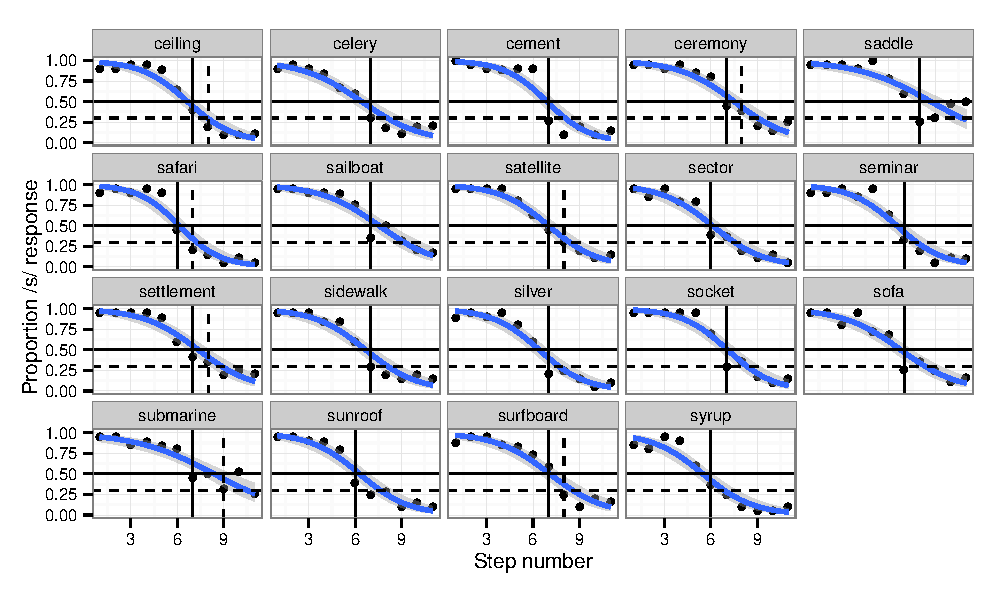
\includegraphics[width=\textwidth]{graphs/sinitialpretest.pdf}
\end{center}
\end{figure*}

\begin{table}
\caption{Step chosen for each Word-initial stimulus in Experiment 1 and the proportion /s/ response in the pretest}
\label{tbl:exp1srespinitial}
\centering
\begin{tabular}{ccc}
\toprule
Word & Step chosen & Proportion /s/ response \\
\midrule
 ceiling & 7 & 0.40 \\
celery & 7 & 0.30 \\
cement & 7 & 0.26 \\
ceremony & 7 & 0.44 \\
saddle & 8 & 0.25 \\
safari & 6 & 0.45 \\
sailboat & 7 & 0.35 \\
satellite & 7 & 0.45 \\
sector & 6 & 0.39 \\
 seminar & 7 & 0.33 \\
 settlement & 7 & 0.42 \\
 sidewalk & 7 & 0.30 \\
 silver & 7 & 0.21 \\
 socket & 7 & 0.30 \\
 sofa & 7 & 0.26 \\
 submarine & 7 & 0.45 \\
 sunroof & 6 & 0.39 \\
 surfboard & 7 & 0.59 \\
 syrup & 6 & 0.37 \\
\midrule
 Average &  6.8 & 0.36 \\

\bottomrule
\end{tabular}
\end{table}

The proportion of /s/-responses (or word responses for exposure items) at each step of each continuum was calculated and the most ambiguous step chosen. 
The threshold for the ambiguous step for Experiment 1 was when the percentage of /s/-response dropped near 50\%. 
The lists of steps chosen for Word-initial target stimuli is in Table~\ref{tbl:exp1srespinitial} and Table~\ref{tbl:exp1srespfinal}, respectively.
For the minimal pairs, six steps surrounding the 50\% cross-over point were selected for use in the phonetic categorization task.  
Due to experimenter error, the continuum for \emph{seedling} was not included in the stimuli, so the chosen step was the average chosen step for the /s/-initial words.  
The average step chosen for Word-initial /s/ words was 6.8 ($SD = 0.5$), and for Word-medial /s/ words the average step was 7.7 ($SD = 0.8$).


\begin{figure*}[ht]
\caption{Proportion of word-responses for Word-medial exposure words. Solid lines represent Experiment 1 selection criteria (50\% word-response rate) and dashed lines represent Experiment 2 selection criteria (30\% word-response rate).  Dots are averaged word-response across subjects, and the blue line is a binomial model constructed from the responses.}
\label{fig:sfinalpretest}
\begin{center}
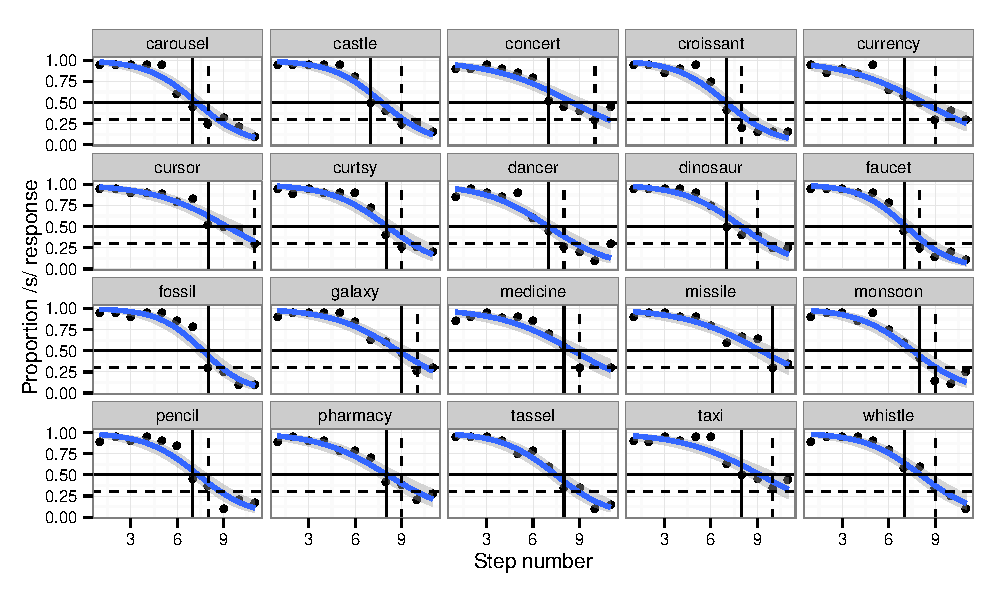
\includegraphics[width=\textwidth]{graphs/sfinalpretest.pdf}
\end{center}
\end{figure*}


\begin{table}
\caption{Step chosen for each Word-medial stimulus in Experiment 1 and the proporation /s/ response in the pretest}
\label{tbl:exp1srespfinal}
\centering
\begin{tabular}{cccc}
\toprule
 Word & Step chosen & Proportion /s/ response \\
\midrule
carousel & 7 & 0.45 \\
castle & 7 & 0.50 \\
concert & 7 & 0.53 \\
croissant & 7 & 0.42 \\
currency & 7 & 0.58 \\
cursor & 8 & 0.53 \\
 curtsy & 8 & 0.40 \\
 dancer & 7 & 0.45 \\
 dinosaur & 7 & 0.50 \\
 faucet & 7 & 0.45 \\
 fossil & 8 & 0.30 \\
 galaxy & 9 & 0.47 \\
 medicine & 8 & 0.55 \\
 missile & 10 & 0.30 \\
 monsoon & 8 & 0.42 \\
 pencil & 7 & 0.45 \\
pharmacy & 8 & 0.42 \\
tassel & 8 & 0.35 \\
 taxi & 8 & 0.50 \\
 whistle & 7 & 0.58 \\
\midrule
 Average   & 7.7 & 0.45 \\

\bottomrule
\end{tabular}
\end{table}

To visualize the effect of morphing on the acoustics of the sibilants and to confirm the desired effects, a multidimensional scaled plot of acoustic distance was constructed.  
Using the \texttt{python-acoustic-similarity} package \citep{McAuliffe2015}, sibilants were transformed into arrays of mel-frequency cepstrum coefficients (MFCC), and then pairwise distances were computed via dynamic time warping to create a distance matrix of the sibilant productions.  
This distance matrix was then multidimensionally scaled to produce Figure~\ref{fig:exp1mds}.  
As seen there, the original, unsynthesized productions (in blue) form four quadrants based on the two principal components of the distance matrix. 
 The first dimension is associated with the centroid frequency of the sibilant, separating /s/ tokens from /\textesh/.  
The second dimension separates out the word-medial sibilants (in smaller font) from the word-initial sibilants (in larger font), likely due to the different coarticulatory effects based on word position.  
The categorization tokens (all word-initial) predictably occupy the space between the word-initial /s/ tokens and the word-initial /\textesh/ tokens. 
 The exposure tokens pattern as expected.  Exposure /\textesh/ tokens are overlapping with the original distributions for /\textesh/ tokens.  
Exposure /s/ tokens are in between /s/ and /\textesh/, though word-medial /s/ tokens are closer to the original /\textesh/ distribution, reflecting the difference in average stimuli step chosen in Tables~\ref{tbl:exp1srespinitial} and~\ref{tbl:exp1srespfinal}.

\begin{figure*}[ht]
\caption{Multidimensional scaling of the acoustic distances between the sibilants of original productions, categorization tokens and the exposure tokens in Experiment 1.  Categorization and exposure tokens were synthesized from the original productions using STRAIGHT \citep{Kawahara2008}.}
\label{fig:exp1mds}
\begin{center}
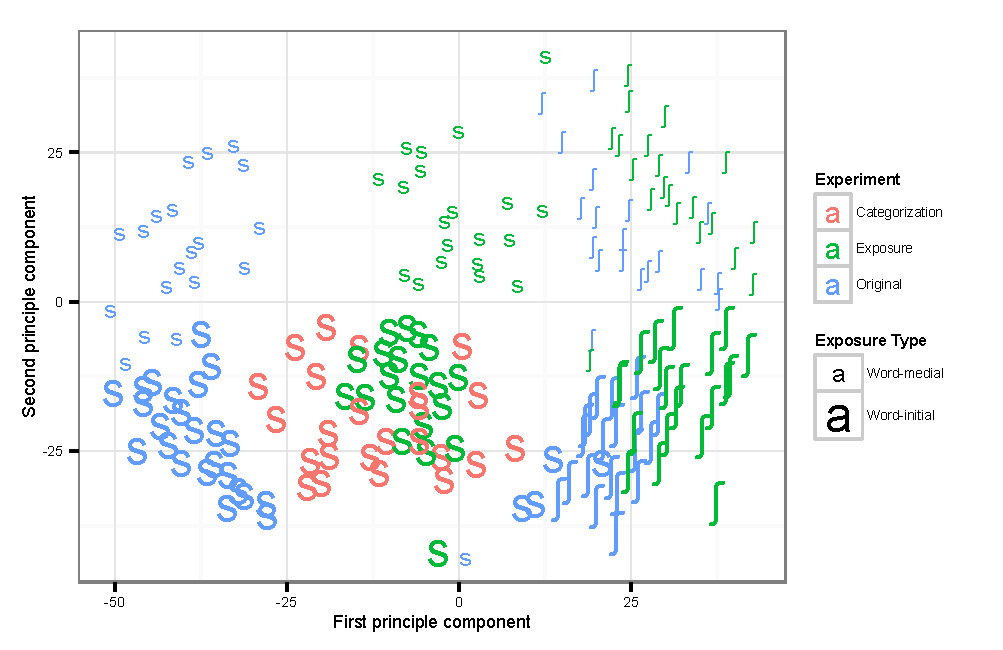
\includegraphics[width=\textwidth]{graphs/exp1_mds}
\end{center}
\end{figure*}

\subsubsection{Procedure}

Participants in the experimental conditions completed an exposure task and a categorization task.  
Exposure was a lexical decision task, where participants heard auditory stimuli and were instructed to respond with either ``word'' if they thought what they heard was a word or ``nonword'' if they did not think it was a word.  
The buttons corresponding to ``word'' and ``nonword'' were counterbalanced across participants. Trial order was pseudorandom, with no critical or control items appearing in the first six trials and no critical or control trials in a row \citep[following][]{Reinisch2013}.
For each trial, a blank screen was shown for 500 ms, and then the two responses and their corresponding buttons on the button box were shown (i.e. "word" and "1" on one side of the screen and "nonword" and "5" on the other side of the screen).
The auditory stimulus was played 500 ms following the presentation of the response options.
Participants had 3000 ms from the onset of the auditory stimulus to respond.
Feedback about whether a response was detected was given once a button was pressed or the 3000 ms had elapsed and was shown for 500 ms before the following trial began.
Every 50 trials participants were given a break and the next trial did not start until the participant pressed a button.

In the categorization task, participants heard an auditory stimulus and had to categorize it as one of two words, differing only in the onset sibilant, i.e. \emph{sin} or \emph{shin}.  
The buttons corresponding to the words were counterbalanced across participants.  
The six most ambiguous steps of the minimal pair continua were used with seven repetitions each, giving a total of 168 trials.
Each trial proceeded similarly to exposure.
A blank screen was displayed for 500 ms, followed by the response screen for 500 ms (i.e. "sin" and "1" on one side, "shin and "5" on the other) before the auditory stimulus was presented.
Participants had 3000 ms from the onset of the auditory stimulus to respond and feedback about whether the response was detected was shown for 1500 ms.
Participants were given a break every 40 trials, except after 160 trials, as that would leave eight trials in the rest of the experiment.

Participants were given oral instructions explaining both tasks at the beginning of the experiment to remove experimenter interaction between exposure and categorization.
Written instructions were presented to participants at the beginning of each task as well.
The instructions for the exposure task given to participants assigned to an Attention condition included explicit reference to the modified sibilants.
Participants were told that ``this speaker's "s" sound is sometimes ambiguous'' and instructed to ``listen carefully so as to choose the correct response.''

\subsection{Results}

\subsubsection{Control experiment}

Responses with reaction times less than 200 ms or greater than 2500 ms were excluded from analyses  \citep[following][]{Reinisch2013}. 
A logistic mixed effects models was fit with Subject and Continuum as random effects and Step as a fixed effect with by-Subject and by-Continuum random slopes for Step. 
The intercept was not significant ($\beta = 0.43, SE = 0.29, z = 1.5, p = 0.13$), and Step was significant ($\beta = -2.61, SE = 0.28, z = -9.1, p < 0.01$).

\subsubsection{Exposure}

Trials with nonword stimuli and responses faster than 200 ms or slower than 2500 ms were excluded from analysis. 
Performance on the exposure task was high overall, with accuracy on filler trials averaging 92\%.  
A logistic mixed-effects model with accuracy as the dependent variable was fit with fixed effects for Trial (0-200), Trial Type (Filler, /s/, and /\textesh/), Attention (No Attention and Attention), Exposure Type (Word-Initial and Word-Medial), and their interactions.   Trial Type was coded using treatment (dummy) coding, with Filler as the reference level.  
Deviance contrast coding was used for Exposure Type (Word-initial = 0.5, Word-medial = -0.5) and Attention (No attention = 0.5, Attention = -0.5).
The random effect structure was as maximally specified as possible with random intercepts for Subject and Word, and by-Subject random slopes for Trial, Trial Type, and their interactions and by-Word random slopes for Attention, Exposure Type, and their interactions. 

A significant fixed effect was found for Trial Type of /s/ versus Filler ($\beta = -2.13, SE = 0.31, z = -6.8, p < 0.01$), as participants were less likely to endorse words containing the modified /s/ category as compared to filler words.
However, there was a significant interaction between Trial and Trial Type of /s/ versus Filler ($\beta = -0.45, SE = 0.14, z = 3.1, p = 0.01$), so the differences in accuracy between words with /s/ and filler words diminished over time.
There was also a significant main effect of Attention ($\beta = -0.57, SE = 0.28, z = -2.0, p = 0.04$), indicating that participants were more accurate at identifying words in the Attention condition compared to the No Attention condition.
However, there was a marginal interaction between Attention and Trial Type of /s/ versus Filler ($\beta = 0.72, SE = 0.39, z = 1.8, p = 0.06$), suggesting that attention only increased accuracy for words not containing the modified /s/ category.
Figure~\ref{fig:exp2exposeacc} shows within-subject mean accuracy across exposure, with Trial in four blocks.

\begin{figure*}[!ht]
\caption{Within-subject mean accuracy for words in the exposure phase of Experiment 1, separated out by Trial Type (Filler, /s/, and /\textesh/). Error bars represent 95\% confidence intervals.}
\label{fig:exp2exposeacc}
\begin{center}
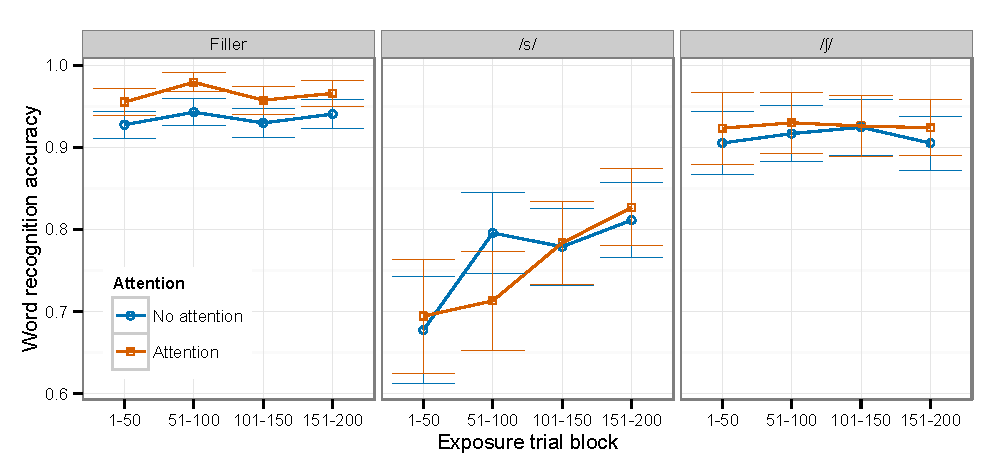
\includegraphics[width=\textwidth]{graphs/exp1_expacc}
\end{center}
\end{figure*}

A linear mixed-effects with logarithmically-transformed reaction time as the dependent variable was fit with identical fixed effect and random effect structure as the logistic model for accuracy.
Significant effects were found for Trial Type of /s/ versus Filler ($\beta = 0.71, SE = 0.07, t = 10.8$) and the interaction between Trial and Trial Type of /s/ versus Filler ($\beta = -0.08, SE = 0.02, t = -3.1$).  
These effects follow the pattern found in the accuracy model, where participants begin with slower reaction times to words with /s/, but over time this difference between words /s/ and filler words lessens.  
Figure~\ref{fig:exp2exposert} shows within-subject mean reaction time across exposure, with Trial in four blocks.

\begin{figure*}[!ht]
\caption{Within-subject mean reaction time to words in the exposure phase of Experiment 1, separated out by Trial Type (Filler, /s/, and /\textesh/). Error bars represent 95\% confidence intervals.}
\label{fig:exp2exposert}
\begin{center}
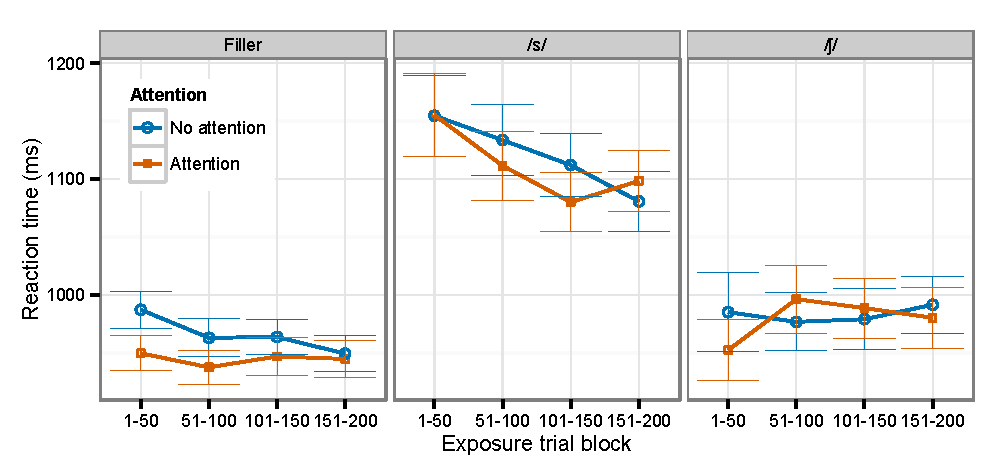
\includegraphics[width=\textwidth]{graphs/exp1_exprt}
\end{center}
\end{figure*}

\subsubsection{Categorization}

Responses with reaction times less than 200 ms or greater than 2500 ms were excluded from analyses. 
Two participants were excluded because their initial estimated cross-over point for the continuum lay outside of the 6 steps presented.  
A logistic mixed effects model was constructed with Subject and Continuum as random effects and a by-Subject random slope for Step and by-Continuum random slopes for Step, Attention, Exposure Type, and their interactions. 
Fixed effects for the model were Step, Exposure Type, Attention, and their interactions.  
Deviance contrast coding was used for Exposure Type (Word-initial = 0.5, Word-medial = -0.5) and Attention (No attention = 0.5, Attention = -0.5).
An /s/ response was coded as 1 and an /\textesh/ response as 0.

\begin{figure*}[!ht]
\caption{Proportion /s/ response along the 6 step continua as a function of Exposure Type and Attention in Experiment 1.    Error bars represent 95\% confidence intervals.}
\label{fig:exp1categ}
\begin{center}
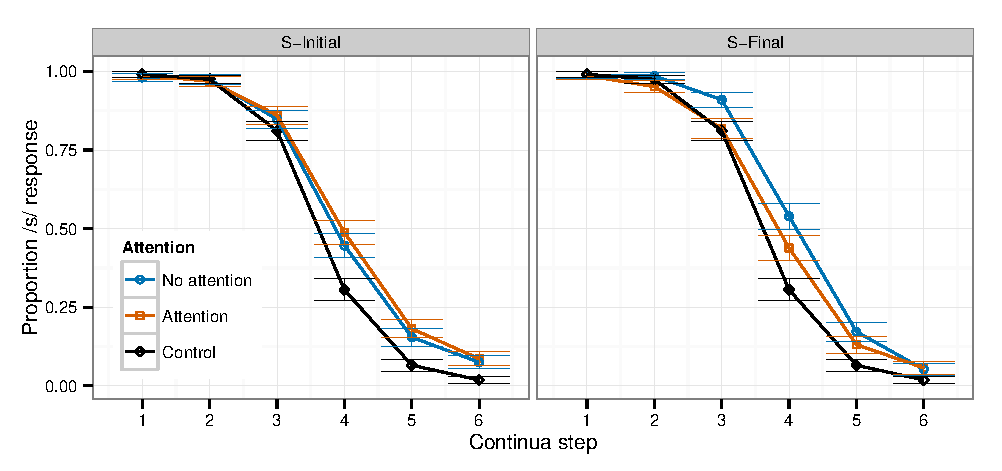
\includegraphics[width=\textwidth]{graphs/exp1_categresults}
\end{center}
\end{figure*}

There was a significant effect for the intercept ($\beta = 0.76, SE = 0.22, z = 3.3, p < 0.01$), indicating that participants categorized more of the continua as /s/ in general.  
This is evidence of learning compared to participants in the control experiment.
There was also a significant main effect of Step ($\beta = -2.14, SE = 0.15, z = -14.2, p < 0.01$), and a significant interaction between Exposure Type and Attention ($\beta = -0.93, SE = 0.45, z = -2.04, p = 0.04$).  The results are visualized Figure~\ref{fig:exp1categ}.
When exposed to a modified /s/ category at the beginning of words, participants show a general expansion of the /s/ category with no difference in behaviour induced by the attention manipulation.  
However, when the exposure is to ambiguous /s/ tokens later in the words, we can see differences in behaviour beyond the general /s/ category expansion.  
Participants not warned of the speaker's ambiguous tokens categorized more of the continua as /s/ compared to those who were warned of the speaker's ambiguous /s/ productions.

\subsection{Discussion}

The condition that showed the largest perceptual learning effect was the one most biased toward a comprehension-oriented attentional set.
Participants exposed to the modified /s/ category in the middle of words and with no explicit instructions about /s/ had larger perceptual learning effects than any of the other conditions.
The other conditions showed roughly equivalent sizes of perceptual learning, suggesting that there was not a compounding effect of explicit attention and word position.
That is, the comprehension-oriented nature of the primary task still exerts an effect on attentional set selection, and a significant perceptual learning effect was found on novel words.

The findings of this experiment do not support the predictions of a purely gain-based mechanism for attention, such as the one posited by \citet{Clark2013}.
If attention functioned as a gain mechanism, increasing the weight of error signals generated by mismatches between expectations and incoming signals, we should expect to see greater perceptual learning when listeners were instructed to attend to the speaker's /s/ sounds.
Instead, the opposite was found.
Participants told to attend to the speaker's /s/ sounds showed smaller perceptual learning effects.
The nature and valency of the instructions may affect the outcome of attention.
In this experiment, the instructions regarding /s/ were phrased to suggest that the ambiguity of the speaker's ``s'' could harm accuracy.
If the valency of the attention were more positive, such as giving an explanation for the cause of ambiguity, then explicit instructions might cause a different pattern of effect.
For a gain-based mechanism, however, valency of attention is not predicted to affect attention, but rather attention always increasing the gain of error signals.
If valency of the instructions does change behaviour, then it would be another mark against a gain mechanism.

In addition to the perceptual learning effects of the categorization phase, the exposure phase also demonstrates learning.  
In the initial trials, words with a modified /s/ are responded to more slowly and less accurately, but over the course of exposure, both reaction times and accuracy approach those of filler and unmodified /\textesh/ words.
Interestingly, only the attention manipulation had an effect on exposure performance, with participants attending to the /s/ category responding more accurately overall.
Exposure Type did not significantly influence accuracy or reaction time in the exposure task.

Much of the literature on perceptual learning in speech perception focuses on the issue of generalization and specificity.
For instance, listeners have been shown to generalize across speakers more if the exposure speaker's modified category happens to be within the range of variation of the categorization speaker's stimuli \citep{Eisner2005,Kraljic2005}.
Additionally, many perceptual learning studies artificially enhance the similarity between exposure tokens and categorization tokens, for instance splicing the maximally ambiguous step of the categorization continuum into expsoure words \citep{Norris2003}.
Because exposure-specificity plays such a large role in perceptual learning, it is natural to consider whether the greater perceptual learning effects in some conditions arise due to greater similarity to the exposure stimuli.
However, as shown in Figure~\ref{fig:exp1mds}, Word-medial exposure tokens are acoustically farther from the categorization tokens than the Word-initial exposure tokens.  
Even if auditory similarity of /s/ across exposure and categorization played any role, it was still overriden by the experimental manipulations.

In this experiment I used a similar method for exposure stimuli selection as \citet{Reinisch2013}, but used a threshold of 50\% word response rate in the pretest as the cutoff rather than 70\%.
With these 70\% stimuli, Reinisch and colleagues report word endorsement rates that consistently exceeded 85\%.
In contrast, Experiment 1 used 50\% as the threshold and had correspondingly lower word endorsement rates (mean = 76\%, sd = 22\%).  
Despite the lower word endorsement rates and the less canonical stimuli used, perceptual learning effects remained robust.
This raises the question, can perceptual learning occur from a modified category even more atypical than the one used in this experiment?
More atypical categories should be more salient and induce more a perception-oriented attentional set, and therefore result in smaller perceptual learning effects.
In Experiment 2, we test whether a comprehension-oriented attentional set can be maintained despite the category atypicality triggering perception-oriented attentional sets.

\section{Experiment 2}

Experiment 2 uses stimuli that are farther from the canonical productions of the critical exposure tokens containing /s/.

\subsection{Methodology}

\subsubsection{Participants}

A total of 127 participants from the UBC population completed the experiment and were compensated with either \$10 CAD or course credit.  
The data from 31 non-native speakers of English were excluded from the analyses.
This left data from 96 participants for analysis.

\subsubsection{Materials}

Experiment 2 used the same items as Experiment 1, except that the step along the /s/-/\textesh/ continua chosen as the ambiguous sound had a different threshold.  
For this experiment, 30\% identification as the /s/ word was used the threshold. The average step chosen for /s/-initial words was 7.3 ($SD = 0.8$), and for /s/-medial words the average step was 8.9 ($SD = 0.9$).  
The list of steps chosen for Word-initial and Word-medial target stimuli are in Tables~\ref{tbl:exp2srespinitial} and~\ref{tbl:exp2srespfinal}, respectively.  
Note that for several stimuli, the same steps are used for both Experiment 1 and 2.
There were large jumps in proportion /s/ response between steps for the continua for those stimuli.
However, the key aspect of the stimuli is the distribution of the /s/ category as a whole, and not the individual steps.

\begin{table}
\caption{Step chosen for each Word-initial stimulus in Experiment 2 and the proportion /s/ response in the pretest}
\label{tbl:exp2srespinitial}
\centering
\begin{tabular}{ccc}
\toprule
 Word & Step chosen & Proportion /s/ response \\
\midrule
 ceiling & 8 & 0.20 \\
 celery & 7 & 0.30 \\
 cement & 7 & 0.26 \\
 ceremony & 8 & 0.39 \\
 saddle & 8 & 0.25 \\
 safari & 7 & 0.21 \\
 sailboat & 7 & 0.35 \\
satellite & 8 & 0.30 \\
 sector & 6 & 0.39 \\
 seminar & 7 & 0.33 \\
 settlement & 8 & 0.35 \\
 sidewalk & 7 & 0.30 \\
 silver & 7 & 0.21 \\
 socket & 7 & 0.30 \\
 sofa & 7 & 0.26 \\
 submarine & 9 & 0.32 \\
 sunroof & 6 & 0.39 \\
 surfboard & 8 & 0.25 \\
 syrup & 6 & 0.37 \\
\midrule
Average  & 7.3 & 0.30 \\

\bottomrule
\end{tabular}
\end{table}


\begin{table}
\caption{Step chosen for each Word-medial stimulus in Experiment 2 and the proportion /s/ response in the pretest}
\label{tbl:exp2srespfinal}
\centering
\begin{tabular}{ccc}
\toprule
 Word & Step chosen & Proportion /s/ response \\
\midrule
 carousel & 8 & 0.25 \\
 castle & 9 & 0.25 \\
 concert & 10 & 0.30 \\
 croissant & 8 & 0.20 \\
 currency & 9 & 0.30 \\
 cursor & 11 & 0.30 \\
 curtsy & 9 & 0.26 \\
 dancer & 8 & 0.26 \\
 dinosaur & 9 & 0.39 \\
 faucet & 8 & 0.25 \\
 fossil & 8 & 0.30 \\
 galaxy & 10 & 0.26 \\
 medicine & 9 & 0.30 \\
missile & 10 & 0.30 \\
monsoon & 9 & 0.15 \\
 pencil & 8 & 0.37 \\
 pharmacy & 9 & 0.39 \\
 tassel & 8 & 0.35 \\
 taxi & 10 & 0.35 \\
 whistle & 9 & 0.35 \\
\midrule
 Average  & 8.9 & 0.29 \\

\bottomrule
\end{tabular}
\end{table}

Multidimensional scaling was employed to assess the distributions of the stimuli used in Experiment 2.
A similar pattern is found for Experiment 2 as Experiment 1.
The axes remain the same as before, with the first dimension corresponding to differences between sibilants, and the second dimension corresponding to differences in word position.
The original productions, categorization tokens, and /\textesh/ tokens in Figure~\ref{fig:exp2mds} are identical to those shown in Figure~\ref{fig:exp1mds}, but the exposure token distribution is shifted towards the /\textesh/ distribution.  
In the Word-medial position, the distributions of /s/ and /\textesh/ are close to overlapping, and in the Word-initial position, they are still separated, but closer than in the stimuli for Experiment 1.


\begin{figure*}[ht]
\caption{Multidimensional scaling of the acoustic distances between the sibilants of original productions, categorization tokens and the exposure tokens in Experiment 2.  Categorization and exposure tokens were synthesized from the original productions using STRAIGHT \citep{Kawahara2008}.}
\label{fig:exp2mds}
\begin{center}
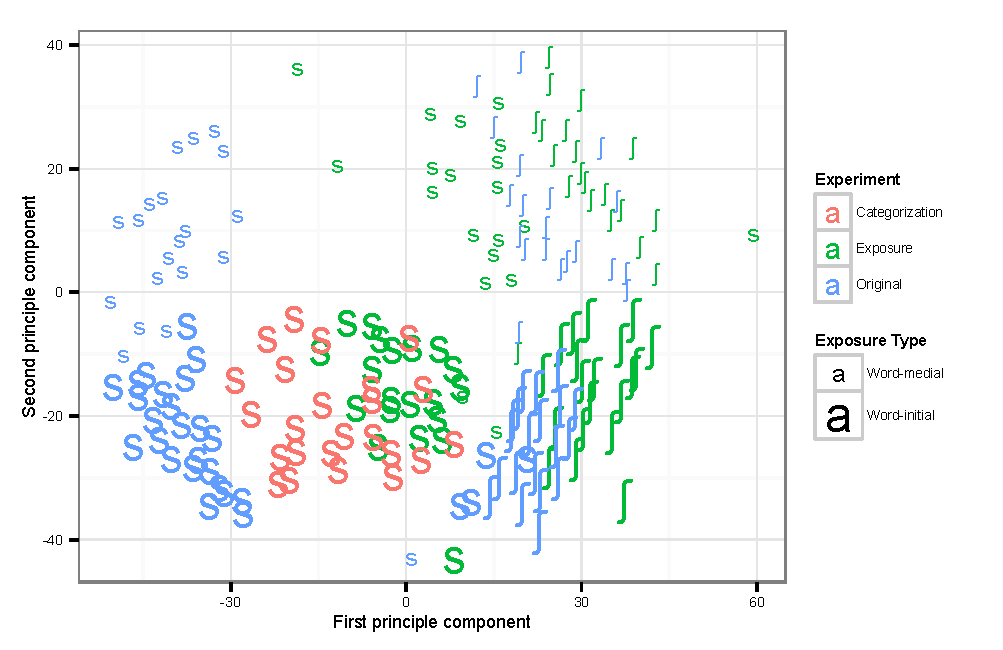
\includegraphics[width=\textwidth]{graphs/exp2_mds}
\end{center}
\end{figure*}

\subsubsection{Procedure}

The procedure and instructions were identical to those of Experiment 1.

\subsection{Results}

\subsubsection{Exposure}

Trials with nonword stimuli and responses faster than 200 ms or slower than 2500 ms were excluded from analysis. 
Performance on the exposure task was as high, with accuracy on filler trials averaging 92\%.  
A logistic mixed-effects model with accuracy as the dependent variable and a linear mixed-effects model with logarithmically-transformed reaction time as the dependent variable were fit with identical specifications as Experiment 1.

In the logistic mixed-effects model of accuracy, a significant fixed effect was found for Trial Type of /s/ versus Filler ($\beta = -3.56, SE = 0.31, z = -11.4, p < 0.01$), with participants less likely to respond that an item was a word if it contained the modified /s/ category.
There was a significant interaction between Trial and Trial Type of /s/ versus Filler ($\beta = -0.29, SE = 0.11, z = 2.5, p < 0.01$) and between Trial and Trial Type of /\textesh/ versus Filler ($\beta = -0.33, SE = 0.16, z = -2.0, p = 0.04$).  
These interactions indicate that participants became more likely to endorse words with modified /s/ productions over time, but also became less accurate on words containing /\textesh/.  
Figure~\ref{fig:exp2exposeacc} shows within-subject mean accuracy across exposure, with Trial in four blocks.

%Trial Type of /s/ versus Filler and Exposure Type ($\beta = 0.97, SE = 0.53, z = 1.8, p = 0.07$) 

\begin{figure*}[!ht]
\caption{Within-subject mean accuracy in the exposure phase of Experiment 2, separated out by Trial Type (Filler, /s/, and /\textesh/). Error bars represent 95\% confidence intervals.}
\label{fig:exp2exposeacc}
\begin{center}
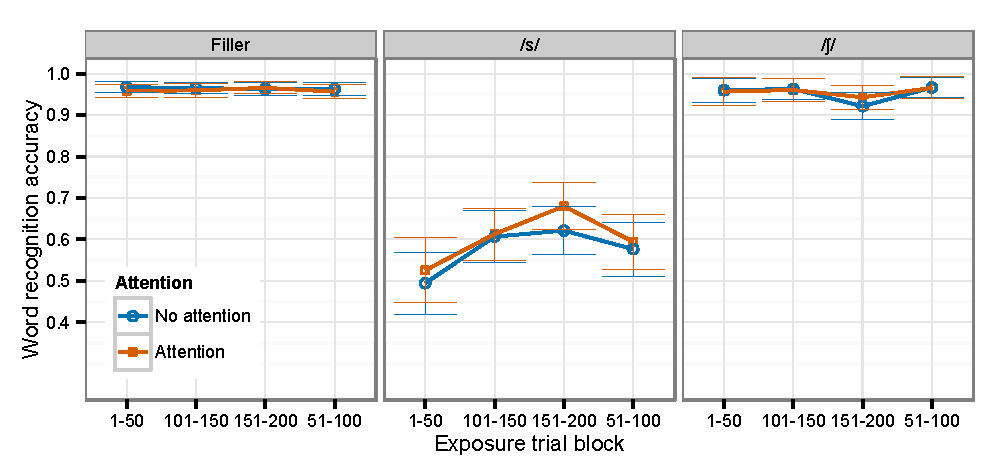
\includegraphics[width=\textwidth]{graphs/exp2_expacc}
\end{center}
\end{figure*}

In the linear mixed-effects model of reaction time, significant effects were found for Trial Type of /s/ versus Filler ($\beta = 0.94, SE = 0.07, t = 14.4$), indicating that reaction times were slower for words containing the modified /s/ category.
Also significant was the interaction between Trial and Trial Type of /\textesh/ versus Filler ($\beta = 0.07, SE = 0.02, t = 3.4$).
However, there was no the interaction between Trial and Trial Type of /s/ versus Filler ($\beta = -0.02, SE = 0.02, t = -0.8$). 
This indicates that reaction time remained relatively stable for words containing the modified /s/ category, but lengthened for words containing the /\textesh/ control.  
There was a marginal effect for Trial Type of /\textesh/ versus Filler ($\beta = 0.14, SE = 0.07, t = 1.9$), indicating that words with /\textesh/ tended to be responded to more slowly than filler times.
Finally, there was a marginal effect of Exposure Type ($\beta = 0.17, SE = 0.09, t = 1.9$), indicating that words in the Word-medial condition tended to be responded to faster.
Figure~\ref{fig:exp2exposert} shows within-subject mean reaction time across exposure, with Trial in four blocks.

%itemtypeSH ($\beta = 0.14, SE = 0.07, t = 1.9$)
%exposure type ($\beta = 0.17, SE = 0.09, t = 1.9$)

\begin{figure*}[!ht]
\caption{Within-subject mean reaction time in the exposure phase of Experiment 2, separated out by Trial Type (Filler, /s/, and /\textesh/). Error bars represent 95\% confidence intervals.}
\label{fig:exp2exposert}
\begin{center}
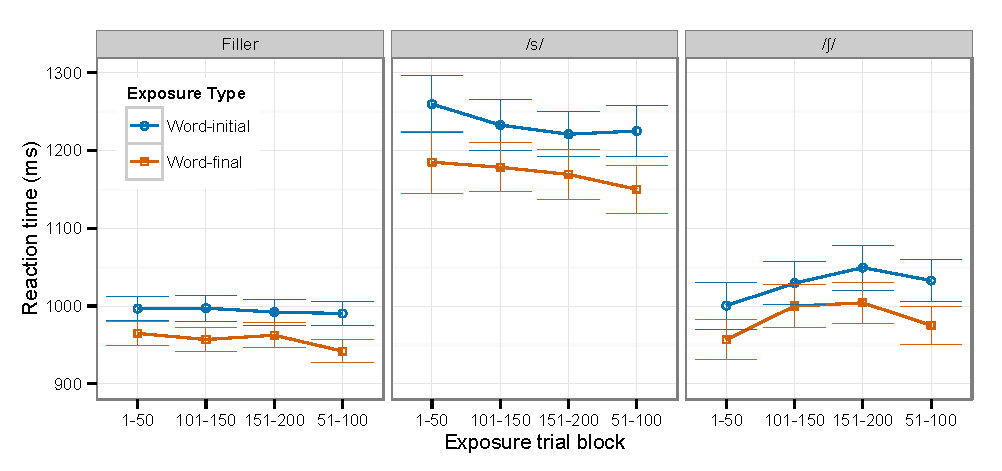
\includegraphics[width=\textwidth]{graphs/exp2_exprt}
\end{center}
\end{figure*}

\subsubsection{Categorization}

Responses with reaction times less than 200 ms or greater than 2500 ms were excluded from analyses. 
Two participants were excluded because their initial estimated cross-over point for the continuum lay outside of the 6 steps presented.  
A logistic mixed effects model was constructed with identical specification as Experiment 1.

\begin{figure*}[!ht]
\caption{Proportion /s/ response along the 6 step continua as a function of Exposure Type and Attention in Experiment 2. Error bars represent 95\% confidence intervals.}
\label{fig:exp2categ}
\begin{center}
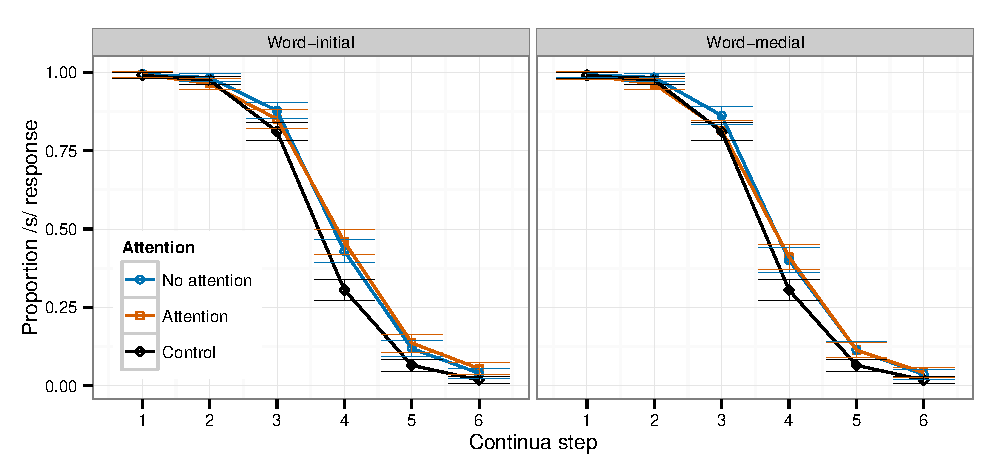
\includegraphics[width=\textwidth]{graphs/exp2_categresults}
\end{center}
\end{figure*}

There was a significant effect for the Intercept ($\beta = 0.60, SE = 0.26, z = 2.3, p = 0.02$), indicating that participants categorized more of the continua as /s/ in general. 
 There was also a significant main effect of Step ($\beta = -2.51, SE = 0.19, z = -13.1, p < 0.01$).  
Unlike in Experiment 1, there were no other significant effects, suggesting that participants across conditions had similar perceptual learning effects.
These results are shown in Figure~\ref{fig:exp2categ}

\section{Grouped results across experiments}

To see what degree the stimuli used had an effect on perceptual learning, the data from Experiment 1 and Experiment 2 were pooled and analyzed identically as above, but with Experiment and its interactions as additional fixed effects.  
In the logistic mixed effects model, there was significant main effects for Intercept ($\beta = 1.00, SE = 0.36, z = 2.7, p < 0.01$) and Step ($\beta = -2.64, SE = 0.21, z = -12.1, p < 0.01$), a significant two-way interaction between Experiment and Step ($\beta = 0.51, SE = 0.20, z = 2.5, p = 0.01$), and a marginal four-way interaction between Step, Exposure Type, Attention and Experiment ($\beta = 0.73, SE = 0.42, z = 1.7, p = 0.08$).  
These results can be seen in Figure~\ref{fig:exp12categ}.  
The four-way interaction can be seen in Word-medial/No Attention conditions across the two experiments, where Experiment 1 has a difference between the Attention and No Attention condition, but Experiment 2 does not.  
The two-way interaction between Experiment and Step and the lack of a main effect for Experiment suggests that while the category boundary was not significantly different across experiments, the slope of the categorization function was.

\begin{figure*}[!ht]
\caption{Proportion /s/ response along the 6 step continua as a function of Exposure Type and Attention in Experiment 1 and Experiment 2. Error bars represent 95\% confidence intervals.}
\label{fig:exp12categ}
\begin{center}
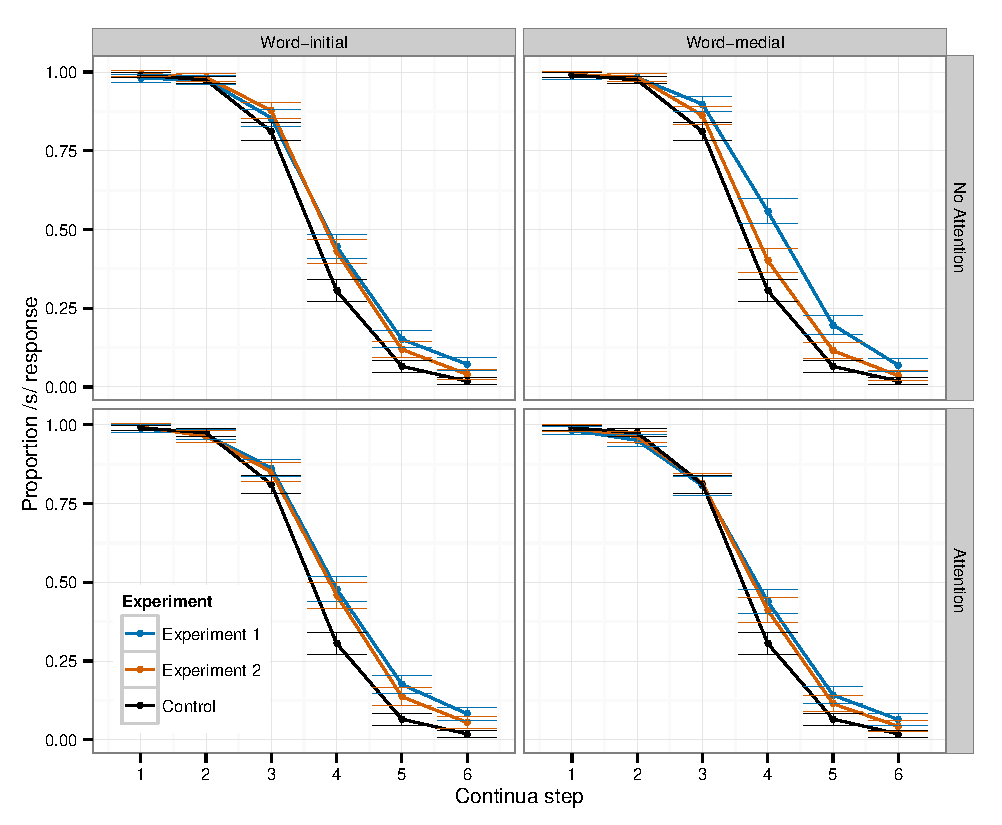
\includegraphics[width=\textwidth]{graphs/exp12_categresults}
\end{center}
\end{figure*}

In previous research, a link has been shown between the proportion of word endorsement for exposure tokens and the size of perceptual learning effects \citep{Scharenborg2013}.
Listeners who endorsed more of exposure tokens as words showed a larger perceptual learning effect.
To assess such a link in the current experiments a logistic mixed-effects model was constructed identically as above, but with participants' word endorsement rate of target /s/ words as an additional fixed effect, along with its interactions with all other fixed effects.
Word endorsement rate was calculated as the ratio of the number of word responses by the total number of /s/ trials (20).
For analysis, the word endorsement rates were analyzed using an arcsine transformation.
Word endorsement rate was significant ($\beta = 1.55, SE = 0.38, z = 4.1, p < 0.01$), finding the same effect as previous work.
Participants who endorsement more exposure tokens showed larger perceptual learning effects.
Word endorsement rate significantly interacted with Step ($\beta = 0.63, SE = 0.24, z = 2.6, p < 0.01$) and was involved in a marginal  interactions with Step, Attention and Experiment ($\beta = -1.79, SE = 0.94, z = -1.8, p = 0.06$).

To better investigate the nature of the four-way interaction, word endorsements were correlated with estimated cross-over points.  
Cross-over points are where a participant's perception switches from predominantly /s/ to predominantly /\textesh/.
The cross-over point was determined from the Subject random intercept and the by-Subject random slope of Step in a simple model containing only those random effects, similar by-Continuum random effects, and a fixed effect for Step \citep{Kleber2012}. 
Scatter plots of word endorsement rate and cross-over point across all experimental conditions are shown in Figure~\ref{fig:exp12xover}.
In general there is a positive correlation between word endorsement rate in the exposure phase and the cross-over point from /s/ to /\textesh/ in the categorization phase.
Participants in the Experiment 1 who were exposed to more typical /s/ stimuli showed a stronger correlation across conditions than participants in Experiment 2 who were exposed to a more atypical /s/ category.
An ANOVA with a dependent variable of word response rate with Exposure Type, Attention, Experiment, and their interactions revealed only a significant difference in endorsement rates for Experiment ($F(1, 187) = 26.8, p < 0.01$).  
Experiment 1 had a mean word endorsment rate of 75\% (SD = 23%) and Experiment 2 had a mean endorsement rate of 58% (SD = 27%).

\begin{figure*}[!ht]
\caption{Correlation of cross-over point in categorization with the proportion of word responses to critical items containing an ambiguous /s/ token in Experiments 1 and 2.}\label{fig:exp12xover}
\begin{center}
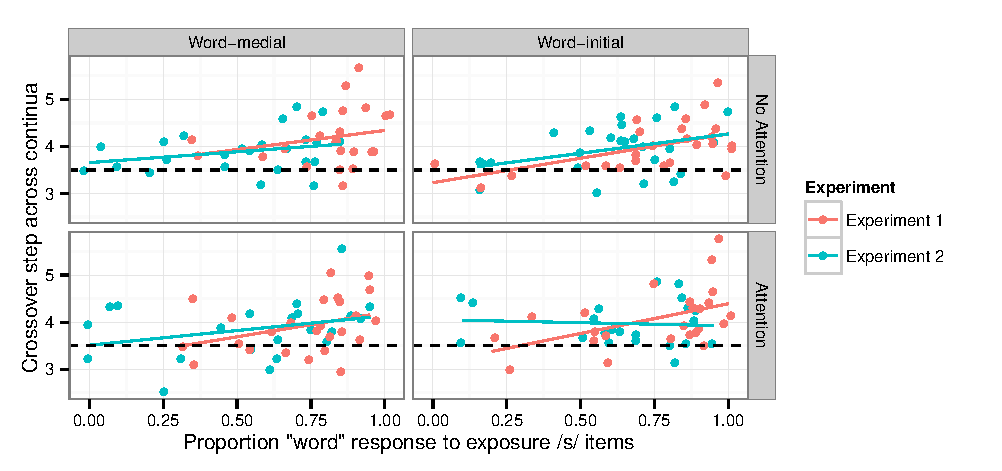
\includegraphics[width=\textwidth]{graphs/exp12_xoverwordresp}
\end{center}
\end{figure*} 

In Experiment 1, the strongest correlations between word endorsement rate and cross-over point are seen in the Word-initial conditions (Attention: $r = 0.46, t(22) = 2.4, p = 0.02$; No Attention: $r = 0.45, t(22) = 2.4, p = 0.02$), with the next strongest, and more marginal, correlation in Word-final/Attention condition ($r = 0.39, t(23) = 2.0, p = 0.06$).  The condition for which the most perceptual learning was observed actually has the weakest correlation ($r = 0.32, t(21) = 1.5, p = 0.13$).

In Experiment 2, the strongest correlation is in the Word-initial/No Attention condition ($r = 0.40, t(23) = 2.1, p = 0.05$), with two trending correlations for the Word-medial conditions (Attention: $r = 0.33, t(20) = 1.6, p = 0.12$; No Attention: $r = 0.27, t(22) = 1.3, p = 0.20$).  Finally, the correlation for the Word-initial/Attention condition is not significant ($r = -0.05, t(20) = -0.2, p = 0.82$).

\section{General discussion}


The perceptual learning effects found in Experiment 1 and 2 align with either comprehension-oriented or perception-oriented attentional sets.  
The perception-oriented attentional sets are predicted to exhibit less generalization, similar to what is seen in psychophysics literature and  in visually-guided perceptual learning in speech perception \citep{Reinisch2014}.
In support of this, participants in Experiment 1 conditions that guided the use of a perception-oriented attentional set (i.e. Attention conditions and Word-initial conditions), showed uniform and modest amounts of perceptual learning.
Those in Experiment 2 who were triggered to use a perception-oriented set based on the category atypicality of the stimuli showed similar modest levels of perceptual learning.
Participants that were not exposed to any triggers towards perception-oriented attentional sets (Experiment 1/ No Attention/ Word-medial) were predicted to use a more comprehension-oriented attentional set which aligns with the task performed.
These participants showed a substantially larger perceptual effect than those bias towards perception-oriented attentional sets.

Compared to Experiment 1, Experiment 2 had a weaker correlation between critical word endorsement rates and cross-over boundary points.
This suggests that although the stimuli used in Experiment 2 were farther from the canonical production, they did not shift the category boundary as much as the stimuli in Experiment 1.  
While neither attention nor position of the ambiguous sound had an effect on the correlation, the distance from the canonical production did.  
This potentially suggests that the degree to which a category is shifted is inversely related to its distance.

In Experiment 1, the decreased correlation between word response rate and cross-over point in the condition that saw the largest perceptual learning effects would fall out from the proposed attention mechanism.
Comprehension-oriented attentional sets are proposed to update higher, more abstract linguistic representations.
Initial endorsements might shift the boundary more than later endorsements under such an attentional set, which would result in a non-linear relationship between endorsement rate and cross-over point.
Lexically-guided perceptual learning is typically induced with relatively few tokens, usually 20 of 200 total tokens \citep{Norris2003, Reinisch2013}, but as few as modified 10 tokens have been shown to cause perceptual learning \citep{Kraljic2008}.
Under perception-oriented attentional sets, the relationship between endorsement rate and cross-over point may be more linear, with equal updating per endorsement, but each individual instance contributes less than initial comprehension-oriented endorsements.
Visually-guided perceptual learning generally uses hundreds of target tokens with no fillers \citep{Vroomen2007, Reinisch2014}.

The correlation between word response rate in the exposure phase and the category boundary in categorization phase across both experiments has two possible explanations. 
In a causal interpretation between exposure and categorization, as each ambiguous sound is processed and errors propagate, the distribution for that category (for that particular speaker) is updated.
Participants who processed more of the ambiguous sound as an /s/ updated their perceptual category for /s/ more. 
This explanation fits within a Bayesian model of the brain \citep{Clark2013} or a neo-generative model of spoken language processing \citep{Pierrehumbert2002}.  
A non-causal story is also plausible:  the correlation may reveal individual differences on the part of the participants, where some participants are more adaptable or tolerant of variability than others.
These more tolerant listeners then show greater degrees of perceptual adaptation. 
Individual differences in attention-switching control have previously been found to affect perceptual learning \citep{Scharenborg2014}, which supports a non-causal interpretation as well.

As mentioned in the discussion for Experiment 1, the findings do not support a simple gain mechanism for attention \citep[contra][]{Clark2013}.  
In \citet{Yeshurun1998}, attention to areas with finer spatial resolution caused observers to miss larger patterns.  
If attention simply boosted the error signal, attention of all kinds should always be beneficial to perceptual learning.
The findings of these two experiments supports a larger role for attention in a predictive coding framework, which been previously noted in \citet{Block2013}.
The propagation-limiting attention mechanism proposed in this dissertation explains both the findings in the visual domain and the current findings.
Attention to a level of representation causes errors between expectations and observed signals to be resolved and updated at that level.
If attention is more oriented towards comprehension, errors can be propagated to a higher, more abstract level of linguistic representation before updating expectations.

In and of itself, a lexical decision task biases a participant towards a comprehension-oriented attentional set.
The experimental manipulations induced perception-oriented attentional sets that attenuated generalized perceptual learning effects.
To fully examine the use of perception- and comprehension-oriented attentional sets in perceptual learning, manipulations that induce comprehension-oriented attentional sets are necessary.
In the following chapter, such a manipulation is implemented through increasing linguistic expectations with semantic predictability.





%% The following is a directive for TeXShop to indicate the main file
%%!TEX root = diss.tex

\chapter{Cross-modal word identification}
\label{chap:sent}

%This chapter investigates perceptual learning with a different bias than lexical, by using sentential context to bias participants towards a particular word.

\section{Motivation}

The largest perceptual learning effect was found in Experiment 1 in the No Attention/ Word-medial condition, which is the condition that was the least likely to promote a perception-oriented attentional set in listeners.
As the lexical decision task is oriented towards comprehension, those in the No Attention/Word-medial group would have maintained a comprehension-oriented attentional set. 
The experiment in this chapter examines perceptual learning in larger sentence contexts, as opposed to lexically guided perceptual learning in single word paradigms.
Using sentences ending with final target words containing a modified /s/ category, semantic predictability is used in conjunction with lexical bias to boost linguistic expectations.
The linguistic expectation exploited in Chapter~\ref{chap:lexdec} was a lexical expectation.
Hearing part of a word increases a listener's expectation for hearing the rest of that word.
But as the words are presented in isolation in the lexical decision task, all words have equal likelihood of occurring, and so no particular expectations are present prior to hearing the initial sounds of the word.
In a sentence context, however, expectations of a particular word can be boosted by the words preceding it.
If the expectation for a word is increased, the expectations for the sounds within it would be increased as well.


For our purposes, semantic predictability refers to how predictable the final word in a sentence is \citep{Kalikow1977}.
Example (1) is a high predictability sentence and Example (2) is an unpredictable sentence.
Although the final word is the same in both, the preceding sentence cues the final word in the predictable sentence, but not in the unpredictable one.
Semantic predictability does not reference formal models of semantics explicitly, but is rather more about world knowledge.

\ex[exno=1]
The cow gave birth to the calf.
\xe
\ex[exno=2,aboveexskip=0pt]
She is glad Jane called about the calf.
\xe


In general, high predictability sentences contain less signal information, but are easier to process and understand.
For example, semantic predictability in production studies is associated with phonetic reduction (particularly duration of words and sounds) independent of lexical factors like frequency and neighborhood density \citep{Scarborough2010, Clopper2008}.  
In speech perception work, semantic predictability and lexical bias been found to have similar effects on phoneme categorization \citep{Connine1987,Borsky1998}.
Sentences with higher semantic predictability are more intelligible in noise, particularly for native speakers \citep[and others]{Kalikow1977, Mayo1997, Fallon2002, Bradlow2007}.
In phoneme restoration tasks, semantic predictability increases the bias to respond that a word is intact with noise added (rather having a sound replaced with noise).
This increased bias is coupled with an increased sensitivity to noise addition versus noise replacement for semantically predictable words \citep{Samuel1981}.

\citet{Samuel1981} proposes that high predictability sentences place a lower cognitive load on the perceptual system.  
The lower cognitive load allows for more cognitive resources to be allocated to the primary perception-oriented task, resulting in greater perceptual sensitivity (though with an increased bias towards restoration as well).
\citet{Mattys2011} manipulated cognitive load through easier or harder concurrent visual search tasks during a phoneme categorization task.
Mirroring the phoneme restoration results, Mattys and colleagues found greater perceptual sensitivity in conditions with lower cognitive load.
In both of these cases, the goal of the listener was oriented towards perception.
A lower cognitive load on the perceptual system may allow more cognitive resources (including attention) to be allocated to perception.
In a comprehension-oriented task, lower cognitive load would not necessarily always result in greater perceptual sensitivity. 
If a listener's end goal is not perception of a specific production of a speech sound, then performance on the task would not necessarily be increased by attending further to perception.

There are many possible outcomes for perceptual learning in this experiment.
Many theoretical frameworks do not make explicit predictions about how the perceptual system will be updated in the context of full sentences.
Most models of speech perception end at perception of words.
In a sentence like Example (1), perceiving individual words is likely not the goal.
For instance, independently perceiving the word \emph{to} does not aid in comprehending the meaning of the sentence.
Instead, comprehension is likely more oriented towards the relations between concepts and perceiving phrases or multiword chunks.
If the perceived chunk is larger than a word, are the fine details still as faithfully encoded as for words in isolation?
Even if the fine details are encoded, are they reliable enough evidence for perceptual learning?
The experiment reported here takes a first pass at answering some of these questions and sets the stage for future inquiry into perceptual learning from sentences. 

One promising avenue for exploring this chapter's research questions lies in the reliability of evidence, which has been shown previously to be crucial for perceptual learning \citep{Kraljic2008, Kraljic2008a}.
If ambiguous productions are accompanied by a video of the speaker holding a pen in their mouth, then no perceptual learning is observed \citep{Kraljic2008}.
Likewise, if listeners are first exposed to typical tokens, and then exposed to atypical tokens, no perceptual learning is observed.
If the order is flipped (atypical tokens first), then perceptual learning effects are present \citep{Kraljic2008}.
If there is linguistic context that conditions a greater variability, then modified tokens in those contexts will not cause perceptual learning \citep{Kraljic2008a}.
However, the unlearned modification must lie within the range of variability conditioned by the context.
For /s/ in /st\textturnr/ clusters, where /s/ becomes more /\textesh/ like due to coarticulation, a more /\textesh/-like modification will not be learned.
Presumably, modifications that lay outside of the variability conditioned by the context will still be learned.
Kraljic and colleagues argue from these studies that listeners will attribute variation to the context as much as possible, and only fall back to updating perceptual categories when no other explanation is available.

Extended beyond single words, reliability can be thought of in terms of perceived carefulness of a word production.
In an experimental setting, every stimulus is carefully curated by the experimenter.
However, both in the laboratory and outside, words in isolation are produced longer and more clearly than their counterparts in full sentences.
Words in isolated sentences are going to be produced less clearly than words in isolation (though not necessarily unintelligibly).
Words in spontaneous conversation are likely to be the least clear, as seen in the ``massive reduction'' in the Buckeye corpus \citep{Johnson2004, Dilts2013}.
All of these factors are dependent on aspects of the sentence (focus, clause type, etc.) or of the speech style, so words in casual conversation will be less clear than words in a formal presentation.

From a perception standpoint, the more clear an acoustic token, the more signal information is available to be processed.
Clear tokens typically have longer durations, increased intensity, and more distinct formants \citep{Krause2004}.
A listener would view tokens that were produced more clearly or with greater care as more reliable productions for that speaker.
Listeners have been found to recognize careful and casual speech equally well, but signal information is used more in careful speech \citep{Sumner2015}.
Extending the argument by Kraljic and colleagues would predict that sentences should have less perceptual learning than words in isolation because (some of) the variability of a word's production in a sentence can be attributed to the fact that the item is in a sentence context.
Additionally, given the propensity for acoustic reduction in high predictability contexts \citep{Scarborough2010}, words in predictable sentences would be even less reliable, leading to less perceptual learning.

This all not to say that sentences are an ineffective method of driving perceptual learning than words in isolation.
From the literature on perceptual learning of foreign accents, sentences are extremely useful in learning to perceive nonnatively accented speakers \citep{Bradlow2008}.
For the purposes of learning an accent, sentences are probably better than words in isolation, as the greater context would allow for better identification of the words.
Differences in perceptual learning from native and nonnative speakers can also be seen in the contradictory findings of \citet{Sumner2011} and \citet{Kraljic2008}.
\citet{Sumner2011} found that listeners could update their perceptual categories constantly over the course of the experiment.
In contrast, \citet{Kraljic2008} found that listeners adapted to the first instances of the category that they heard and did not use subsequent tokens.
The nativeness of the exposure speaker differed in the two experiments.
Constant adaptation was found for a nonnative speaker \citep{Sumner2011} rather than a native speaker \citep{Kraljic2008}.
Listeners may be more biased toward typical native categories for native speakers, so that exposure to an initially typical category causes listeners to disregard the later atypical category as unreliable.
In so doing, listeners can leverage their previous experience with native speakers more readily.
Listeners' previous experience does not as readily extend to nonnative speech, where interspeaker and intraspeaker variation is more prevalent, so constant adaptation and consistent token reliability would improve comprehension the most.

This dissertation largely adopts the predictive coding framework presented in \citet{Clark2013} to account for perceptual learning.
Reliability of sensory information is not directly addressed in Clark's exposition.
The basic form of his model, however, predicts that increasing expectations should always increase error signals.
In \citet[cited in \citet{Clark2013}]{Egner2010}, participants who were expecting to see a face in static had equally-sized neuronal responses in the fusiform face area for face stimuli as for non-face stimuli.  
Participants who were not expecting to see faces showed neuronal responses in that area only for the face stimuli.
The mismatch between expectation and the perceived signal generated an error signal of similar magnitude to the signal itself.
If increased expectations result in increased error signals, perceptual learning should be largest for participants exposed to the modified category in higher predictability sentences.
If smaller perceptual learning effects are observed for those participants, then reliability weighting or attribution of error signals would be necessary in the model.

To test these predictions a novel exposure paradigm was used in place of the normal lexical decision task.  
In this paradigm, participants are presented with sentences auditorily.  
Following the sentence, two pictures appear on the screen: one matching the final word of the sentence and the other a distractor. 
Participants are instructed to indicate which picture corresponds to the final word of the sentence.
Following exposure, participants completed the same categorization task as those in Experiments 1 and 2.

\section{Methodology}

\subsection{Participants}

A total of 137 participants from the UBC population completed the experiment and were compensated with either \$10 CAD or course credit.  
The data from 39 nonnative speakers of English were excluded from the analyses.
No participants reported speech or hearing disorders.
This left data from 98 participants for analysis.
Twenty additional native English speakers participated in a pretest to determine sentence predictability, and 10 other native English speakers participated in a picture naming pretest.

\subsection{Materials}

One hundred and twenty sentences were used as exposure materials.  
The set of sentences consisted of 40 critical sentences, 20 control sentences and 60 filler sentences. 
The critical sentences ended in one of 20 of the critical words in Experiments 1 and 2 that had an /s/ in the onset of the final syllable.  
The 20 control sentences ended in the 20 control items used in Experiments 1 and 2, and the 60 filler sentences ended in the 60 filler words in Experiments 1 and 2.  
Half of all sentences were written to be predictive of the final word, and the other half were written to be unpredictive of the final word.  
Unlike previous studies using sentence or semantic predictability \citep{Kalikow1977}, unpredictive sentences were written with a range of sentence structures.
In all cases, the final words were plausible objects of lexical verbs and prepositions.
High and low predictability filler sentences can be found in Tables~\ref{tbl:senthighfiller} and~\ref{tbl:sentlowfiller}, respectively.
High and low predictability filler sentences with /\textesh/ words can be found in Tables~\ref{tbl:senthighsh} and~\ref{tbl:sentlowsh}, respectively.
Finally, high and low predictability critical sentences can be found in Tables~\ref{tbl:senthighs} and~\ref{tbl:sentlows}, respectively.
Aside from the sibilants in the critical and control words, the sentences contained no sibilants (/s z \textesh\ \textyogh\ \textteshlig\  \textdyoghlig/).  
The same minimal pairs for phonetic categorization as in Experiments 1 and 2 were used.

\begin{table}[!ht]
\caption{High predictability filler sentences.}
\label{tbl:senthighfiller}
\small
\centering
\begin{tabular}{llc}
\toprule
Sentence                                                                     & Word        & Distractor  \\
\midrule
The oak tree grew from a tiny                                                & acorn       & pineapple   \\
The radio in the car didn't work with a bent                                 & antenna     & towel       \\
The clown made the girl an animal from a                                     & balloon     & pancake     \\
Everyday the panda had to eat a lot of                                       & bamboo      & boomerang   \\
The belt had an ornate                                                       & buckle      & hamburger   \\
The caterpillar came out of the cocoon a beautiful                           & butterfly   & crayon      \\
The hermit lived in a log                                                    & cabin       & parade      \\
They marked the date on the                                                  & calendar    & antler      \\
They rode to the pyramid on the back of a                                    & camel       & atom        \\
Right before the plane took off,  & & \\
the captain called the flight crew from the & cockpit     & doorknob    \\
The woman threaded the bowtie through her                                    & collar      & ladybug     \\
At the rodeo, the cattle were rounded up by the                              & cowboy      & ripple      \\
The baby rocked in her                                                       & cradle      & telephone   \\
The delivery man rang the                                                    & doorbell    & firewood    \\
He moved the wet laundry over to the                                         & dryer       & hydrant     \\
The tiny rodent terrified the big, grey                                      & elephant    & pepper      \\
The criminal wore a glove to not leave behind one                            & fingerprint & island      \\
The cook needed one more clove of                                            & garlic      & wheelbarrow \\
Red paint in hand, the youth tagged the building with                        & graffiti    & catapult    \\
The watery dinner had to be poured out with a                                & ladle       & lollipop    \\
The man reheated the leftover dinner in the                                  & microwave   & ukulele     \\
Every dinner plate came with a folded                                        & napkin      & toothpick   \\
The ballroom had a grand                                                     & piano       & dolphin     \\
The woman tied her hair back in a                                            & ponytail    & airport     \\
The adult frog developed from a                                              & tadpole     & bucket      \\
The acting company performed in an old                                       & theatre     & earmuff     \\
Her favorite burrito came wrapped in a flour                                & tortilla    & falafel     \\
The farm youth rode around on the                                            & tractor     & barbecue    \\
The train went under a mountain through a                                    & tunnel      & wagon       \\
The heavy rainfall could have been predicted by the                          & weatherman  & robot      \\
\bottomrule
\end{tabular}
\end{table}

\begin{table}[!ht]
\caption{Low predictability filler sentences.}
\label{tbl:sentlowfiller}
\small
\centering
\begin{tabular}{llc}
\toprule
Sentence                                                                     & Word        & Distractor  \\
\midrule
They clapped loudly for the                       & acrobat    & pillow      \\
The man liked to begin the day with an            & apple      & vampire     \\
Wearily, the woman built up her                   & campfire   & bagel       \\
He looked forward to freely available             & candy      & donkey      \\
The couple never agreed on the                    & cutlery    & butter      \\
He took pride in the renovated                    & darkroom   & candle      \\
They were enthralled by the                       & diamond    & kiwi        \\
While he lay on the ground, the boy played with a & feather    & broccoli    \\
To get any farther, they definitely needed a good & goalie     & waterfall   \\
He didn't know how to get to the                  & gondola    & honey       \\
They were a little frightened to board the        & helicopter & cannon      \\
The woman needed to borrow a                      & ladder     & flagpole    \\
He had to track down and get help from the        & librarian  & tornado     \\
They had a good view of the                       & lightning  & coffee      \\
Toward the end, they were running low on          & lumber     & anvil       \\
They liked how it looked on the                   & mannequin  & parrot      \\
On the way, they liked walking through the        & meadow     & cupcake     \\
The couple were looking forward to buying a       & minivan    & tugboat     \\
He finally made it to the                         & motel      & armadillo   \\
They went out for a quick bite to eat after the   & movie      & volleyball  \\
He really liked the look of the                   & mural      & monocle     \\
After a long night, he devoured the whole         & omelet     & hummingbird \\
On the field trip, they learned all about the     & painter    & pulley      \\
The boy cried when they took away the             & popcorn    & puppet      \\
The irate woman yelled at the                     & referee    & propeller   \\
When they were called, the group moved to the     & table      & helmet      \\
He didn't know about a problem with the           & teapot     & crowbar     \\
He had to remember to pick up the                 & tire       & parakeet    \\
Every day he dreaded the late afternoon           & traffic    & rowboat     \\
The woman kept a lookout for the                  & umbrella   & catamaran  \\
\bottomrule
\end{tabular}
\end{table}

Sentences were recorded by the same male Vancouver English speaker used in Experiments 1 and 2.  
Critical sentences were recorded in pairs, with one normal production and then a production of the same sentence with the /s/ in the final word replaced with an /\textesh/.  
The speaker was instructed to produce both sentences with comparable speech rate, speech style, and prosody.

\begin{table}[!ht]
\caption{High predictability sentences with /\textesh/ words.}
\label{tbl:senthighsh}
\small
\centering
\begin{tabular}{llc}
\toprule
Sentence                                                                     & Word        & Distractor  \\
\midrule
The bidding became frantic for the final item in the                     & auction     & accordion  \\
While waiting in line at the new bank,  & & \\
the woman read their introductory & brochure    & blueberry  \\
The woman only got a dime back after paying the                          & cashier     & laptop     \\
He could only kneel for a little while without a plump                   & cushion     & forklift   \\
Lava flowed down the volcano after the violent                           & eruption    & pumpkin    \\
The bear awoke from her winter                                           & hibernation & violin     \\
After jumping out of the plane, the woman opened her                     & parachute   & camera     \\
The doctor took the time to look in on every                             & patient     & crocodile  \\
While down with the flu, the woman invariably carried a clean            & tissue      & whirlpool  \\
The opera-goer found her row with the help of an                         & usher       & doormat   \\
\bottomrule
\end{tabular}
\end{table}

\begin{table}[!ht]
\caption{Low predictability sentences with /\textesh/ words.}
\label{tbl:sentlowsh}
\small
\centering
\begin{tabular}{llc}
\toprule
Sentence                                                                     & Word        & Distractor  \\
\midrule
The woman couldn't wait to fill up the        & bookshelf  & muffin     \\
The whole family travelled for an hour to the & coronation & waffle     \\
He did not look forward to the                & handshake  & raccoon    \\
He gave a wide berth to the                   & machine    & kitten     \\
They dragged their feet on the way to the     & mansion    & treadmill  \\
He had a hard time with                       & meditation & beekeeper  \\
They were deeply worried about the            & militia    & peanut     \\
He went on and on about the                   & milkshake  & elbow      \\
For winter break, he wanted to go to the      & ocean      & iguana     \\
He could finally get a new                    & windshield & koala     \\
\bottomrule
\end{tabular}
\end{table}

\begin{table}[!ht]
\caption{High predictability sentences with target /s/ words.}
\label{tbl:senthighs}
\small
\centering
\begin{tabular}{llc}
\toprule
Sentence                                                                     & Word        & Distractor  \\
\midrule
At the carnival the girl rode a unicorn around the & carousel & pirate \\
A deep moat protected the old & castle & martini \\
The encore from the pop duo perfected the whole & concert & earplug \\
From the bakery he got a flaky, buttery & croissant & windmill \\
After her world trip, & & \\
the traveller had a little money leftover in every local & currency & elevator \\
When the computer locked up, he couldn't move the & cursor & clover \\
The lady returned the bow with a formal & curtsy & gavel \\
The critic raved about the ballet and the lead & dancer & cricket \\
Long ago, a comet hit the earth, killing every big & dinosaur & bandana \\
Water poured into the bath tub from the & faucet & doughtnut \\
After millennia, the bone in the riverbed turned into a & fossil & menorah \\
The name 'Milky Way' can perfectly depict our & galaxy & kayak \\
We no longer worry about the plague due to modern & medicine & cucumber \\
In the heated aerial battle, neither pilot could lock on with a & missile & cookie \\
Rain fell every day in India during the & monsoon & gargoyle \\
The man wrote on the paper with a graphite & pencil & trombone \\
The woman got an over-the-counter drug at her local & pharmacy & kettle \\
From the cap of the new grad hung a golden & tassel & guitar \\
The New Yorker flagged down a & taxi & ribbon \\
The traffic cop alerted the driver by blowing her & whistle & ravioli \\
\bottomrule
\end{tabular}
\end{table}

\begin{table}[!ht]
\caption{Low predictability sentences with target /s/ words.}
\label{tbl:sentlows}
\small
\centering
\begin{tabular}{llc}
\toprule
Sentence                                                                     & Word        & Distractor  \\
\midrule
They got back in line for the & carousel & pirate \\
He dreaded the long walk to the & castle & martini \\
He prepared night and day for the & concert & earplug \\
The man had a craving for a & croissant & windmill \\
They weren't worried about the different & currency & elevator \\
The man could never find the & cursor & clover \\
The girl didn't want to make a & curtsy & gavel \\
The boy wanted to become a better & dancer & cricket \\
The boy really wanted to ride the & dinosaur & bandana \\
The woman hoped to get a working & faucet & doughtnut \\
No one knew where to find the & fossil & menorah \\
The man talked at length about the & galaxy & kayak \\
With that GPA, they could have a career in & medicine & cucumber \\
The boy wanted to build a toy & missile & cookie \\
On their picnic, they avoided the & monsoon & gargoyle \\
The woman looked frantically for her & pencil & trombone \\
The woman loved her work at the & pharmacy & kettle \\
He worried about the color of the & tassel & guitar \\
The woman had no luck getting a & taxi & ribbon \\
The boy ran away when he heard the & whistle & ravioli \\
\bottomrule
\end{tabular}
\end{table}

As in Experiments 1 and 2, the critical items were morphed together into an 11-step continuum using STRAIGHT \citep{Kawahara2008}; only the final word in each sentence was morphed. 
The preceding words were the synthesized versions of the sentence with the correct /s/ production to minimize artifacts of the morphing algorithm.  
The control and filler items were also processed and resynthesized to ensure consistent quality.  
The ambiguous point selection was based on the pretest performed for Experiment 1 and 2 exposure items.  
The ambiguous steps of the continua chosen corresponded to the 50\% cross over point in Experiment 1.

Acoustic distances between exposure tokens, categorization tokens, and their original productions were multidimensionally scaled.  In Figure~\ref{fig:exp3mds}, the original productions are separated again by the first dimension, which corresponds to the centroid frequency of the sibilant.
The categorization tokens are predictably in between the original productions and offset in the second dimension due to their different position in the word.
The exposure tokens for Experiment 3 fit in between the original productions and the categorization tokens.

\begin{figure*}[ht]
\caption{Multidimensional scaling of the acoustic distances between the sibilants of original productions, categorization tokens and the exposure tokens in Experiment 3.}
\label{fig:exp3mds}
\begin{center}
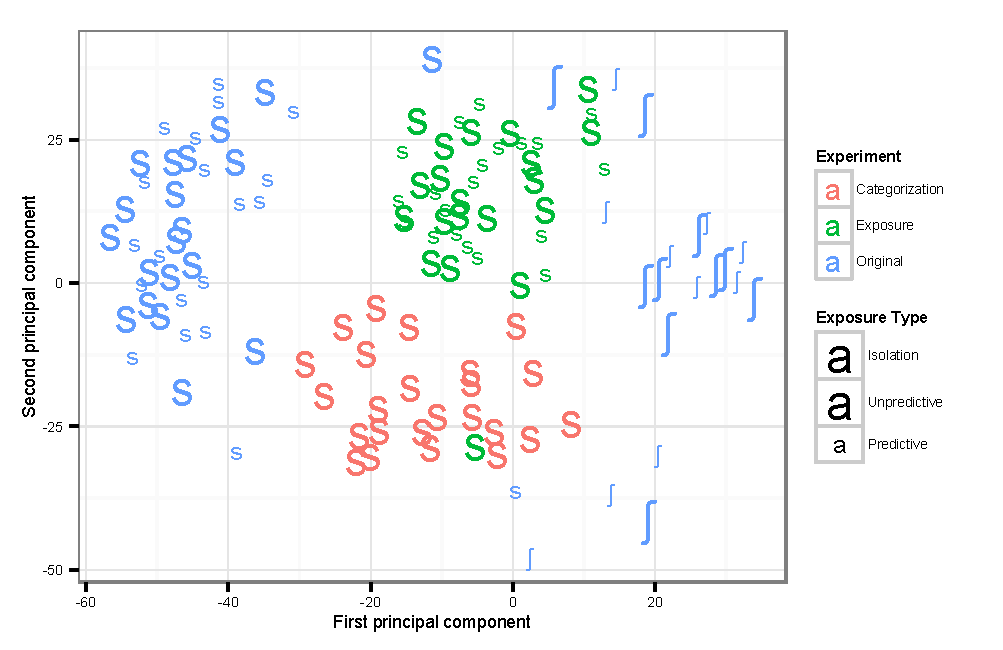
\includegraphics[width=\textwidth]{graphs/exp3_mds}
\end{center}
\end{figure*}

Sentences were pairs with two pictures apiece.
Pictures of 200 words, with 100 pictures for the final word of the sentences and 100 for distractors, were selected in two steps.  
First, a research assistant selected five images from a Google image search of the word, and then a single image representing that word was selected from amongst the five by me.  
To ensure consistent behavior in E-Prime \citep{PsychologySoftwareTools2012}, pictures were resized to fit within a 400x400 area with a resolution of 72x72 DPI and converted to bitmap format.  
Additionally, any transparent backgrounds in the pictures were converted to plain white backgrounds.

\subsection{Pretest}

The same twenty participants that completed the lexical decision continua pre-test also completed a sentence predictability task before the phonetic categorization task described in Experiment 1. 
Participants were compensated with \$10 CAD for both tasks, and were native North American English speakers with no reported speech, language or hearing disorders. 
In this task, participants were presented with sentence fragments that were lacking in the final word.  
These sentence fragments were the 120 sentences to be used as exposure items for the perceptual learning experiment.
Participants were instructed to type in the word that came to mind when reading the fragment, and to enter any additional words that came to mind that would also complete the sentence.  
There was no time limit for entry and participants were shown an example with the fragment ``The boat sailed across the...'' and the possible completions ``bay, ocean, lake, river''.  
Responses were collected in E-Prime \citep{PsychologySoftwareTools2012}, and were sanitized by removing miscellaneous keystrokes, spell checking, and standardizing variant spellings and plural forms.

From the sanitized data, responses were coded as either 0 if the target word was not present or 1 if it was.
For each sentence, the target response rate was calculated by averaging responses from all participants.
The target response rate was 0.49 (range 0-0.95) for predictive sentences and 0.03 (range 0-0.45) for unpredictive sentences.
Predictive sentences that had target response rates of 0.2 or less were rewritten.  
The predictive sentences for \emph{auction}, \emph{brochure}, \emph{carousel}, \emph{cashier}, \emph{cockpit}, \emph{concert}, \emph{cowboy}, \emph{currency}, \emph{cursor}, \emph{cushion}, \emph{dryer}, \emph{graffiti}, and \emph{missile} were rewritten to remove any syntactic or semantic ambiguities.
For instance, a common completion for the predictive sentence ``The youth tagged the wall with...'' was ``spray paint'' rather than ``graffiti''.
To promote the likelihood of ``graffiti'', the sentence was changed to ``Red paint in hand, the youth tagged the wall with...'', which would eliminate ``spray paint'' as a possible completion.

Five volunteers participated in another pretest to determine how suitable the pictures were at representing their associated word.  
All participants were native speakers of North American English, with reported corrected-to-normal vision. Participants were presented with a single image in the middle of the screen.  
Their task was to type the word that first came to mind, and any other words that described the picture equally well.  
There was no time limit and presentation of the pictures was self-paced. Responses were sanitized as above.  

Pictures were replaced if 20\% or less of the participants (1 of 5) responded with the target word and the responses were semantically unrelated to the target word. 
Five pictures were replaced, \emph{toothpick} and \emph{falafel} with clearer pictures and \emph{ukulele}, \emph{earmuff} and \emph{earplug} were replaced with \emph{rollerblader}, \emph{anchor} and \emph{bedroom}.  
All five replacements were for distractor words.

\subsection{Experiment design}

Participants were assigned to one of four groups from a 2x2 between-subject factorial design.
The first factor was whether the word containing the ambiguous sibilant was predictable from the preceding words or not  (Predictability: Predictive versus Unpredictive).
All participants were therefore exposed to a consistent 100 stimulus sentences with identical control and filler items for all participants.
The second factor was whether participants were given additional instructions about the sibilant or not (Attention: Attention versus No Attention).
Participants in the Attention condition received additional instructions that the speaker's ``s'' sounds were sometimes ambiguous, and to listen carefully to ensure correct responses.

\subsection{Procedure}

As in Experiments 1 and 2, participants completed an exposure task and a categorization task in E-Prime \citep{PsychologySoftwareTools2012}.  
For the exposure task, participants heard a sentence via headphones for each trial.  
Immediately following the auditory presentation, they were presented with two pictures on the screen.  
Their task was to select the picture on the screen that corresponded to the final word in the sentence they heard.  
The order was pseudorandom with the same constraints described in Experiment 1.
Half of the matching pictures were selected via one button and half via the other.

Each trial proceeded as follows.
A blank screen was presented for 250 ms.
Immediately following, a sentence was presented auditorily.
Following the auditory stimulus, two pictures and their respective buttons appeared on the screen.
For example, a sentence ending in ``dog'' would show a picture of a dog and ``1'' on one side of the screen, and a picture of a banana and ``5'' on the other side of the screen.
Participants had up to 3000 ms to respond which picture matched the final word in the sentence.
Feedback as to whether a response was detected was shown for 500 ms before the next trial began.
Participants were given a self-paced break after 50 trials.

Following the exposure task, participants completed the same categorization task described in Experiments 1 and 2.

Participants were given oral instructions explaining both tasks at the beginning of the experiment to remove experimenter interaction between exposure and categorization.
Written instructions were presented to participants at the beginning of each task as well.
The instructions for the exposure task given to participants assigned to an Attention condition included explicit reference to the modified sibilants.
Participants were told that ``this speaker's `s' sound is sometimes ambiguous'' and instructed to ``listen carefully so as to choose the correct response.''

\subsection{Analysis}

Response data and factors were transformed and analyzed in the same way as in Experiment 1 and 2.

\section{Results}

\subsection{Exposure}

Performance in the task was high, with accuracy near ceiling across all subjects (mean accuracy = 99.5\%, sd = 0.8\%).
Due to these ceiling effects, a logistic mixed-effects model of accuracy was not constructed.  
A linear mixed effects model for logarithmically-transformed reaction time was constructed with a similar structure as in Experiments 1 and 2.
Fixed effects were Trial (0-100), Trial Type (Filler, /s/, and /\textesh/), Attention (No Attention and Attention), Predictability (Unpredictive and Predictive), and their interactions.  
By-Subject and by-Word random effect structure was as maximal as permitted by the data, with by-Subject random slopes for Trial, Trial Type, Predictability, and their interactions and by-Word random slopes for Attention, Predictability, and their interaction. 
Trial Type was coded using treatment (dummy) coding, with Filler as the reference level. 
Deviance contrast coding was used for Predictability (Unpredictive = 0.5, Predictive = -0.5) and Attention (No attention = 0.5, Attention = -0.5).

\begin{figure*}[!ht]
\centering
\caption{Within-subject mean reaction time in the exposure phase of Experiment 3, separated out by Trial Type (Filler, /s/, and /\textesh/). Error bars represent 95\% confidence intervals.}
\label{fig:exp3exposert}
\begin{center}
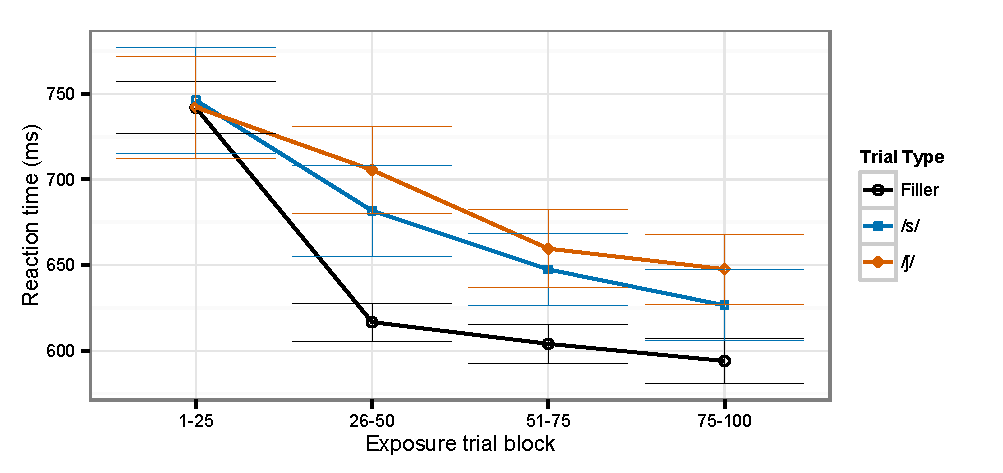
\includegraphics[width=0.95\textwidth]{graphs/exp3_exprt}
\end{center}
\end{figure*}

A significant effect was found for Trial ($\beta = -0.20, SE = 0.01, t = -11.0$), indicating that reaction time became faster over the course of the experiment.
There was a significant effect for Trial Type of /\textesh/ versus Filler ($\beta = 0.19, SE = 0.09, t = 2.1$), but not for /s/ versus Filler ($\beta = 0.11, SE = 0.09, t = 1.3$), suggesting that words with /\textesh/ in them were responded to more slowly than filler words or those with a modified /s/ in them.
There was a significant interaction between Trial and Trial Type of  /s/ versus Filler ($\beta = 0.05, SE = 0.02, t = 2.4$) and between Trial and Trial Type of /\textesh/ versus Filler ($\beta = 0.05, SE = 0.02, t = 2.9$), indicating that reaction time for words with /s/ or /\textesh/ in them did not become as fast across the experiment as those for filler words.
These results are shown in Figure~\ref{fig:exp3exposert}.
Note that the y-axis has a different scale than that used in Experiments 1 and 2 for reactions times.
Participants were faster in general in this task than in the lexical decision task.
Responses to predictable sentences (mean = 669 ms, SD = 321 ms) were not significantly faster than responses to unpredictable sentences (mean = 646 ms, SD = 299 ms), suggesting that performance was at floor.


\subsection{Categorization}

Responses with reaction times less than 200 ms or greater than 2500 ms were excluded from analyses. 
A logistic mixed effects model was constructed with Subject and Continua as random effects and continua Step as random slopes, with 0 coded as a /\textesh/ response and 1 as a /s/ response.  Fixed effects for the model were Step, Exposure Type, Attention, and their interactions, with deviance coding used for contrasts for Exposure Type (Unpredictive = 0.5, Predictive = -0.5) and Attention (No attention = 0.5, Attention = -0.5).


\begin{figure*}[!ht]
\caption{Proportion /s/ response along the 6 step continua as a function of Exposure Type and Attention in Experiment 3.  Error bars represent 95\% confidence intervals.}
\label{fig:exp3categ}
\begin{center}
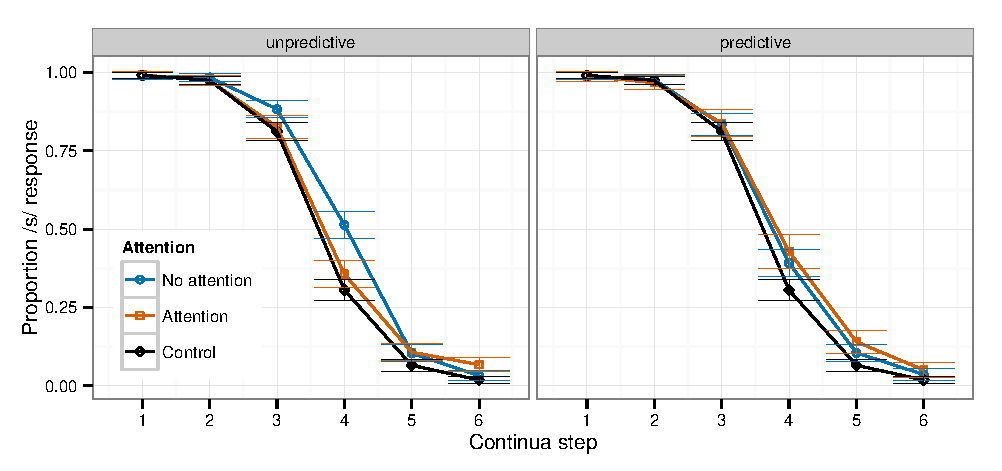
\includegraphics[width=\textwidth]{graphs/exp3_categresults}
\end{center}
\end{figure*}

As in the previous experiments, there was a significant effect of the intercept ($\beta = 0.52, SE = 0.20, z = 2.6, p < 0.01$) and of Step ($\beta = -2.49, SE = 0.19, z = -12.7, p < 0.01$).
Exposure Type ($\beta = 0.23, SE = 0.23, z = 0.97, p = 0.33$), Attention ($\beta = 0.30, SE = 0.21, z = 1.4, p = 0.15$), and their interaction ($\beta = 0.38, SE = 0.44, z = 0.9, p = 0.39$) are all not significant, despite the visible differences in Figure~\ref{fig:exp3categ}.
In Figure~\ref{fig:exp3categ}, there appears to be a similar interaction pattern as was seen for Experiment 1 (Figure~\ref{fig:exp1categ}).
The means for the center steps in the Unpredictive condition appear to be different depending on Attention, while those in the Predictive condition show no such Attention difference.
As will be shown later, the lack of an effect is likely due a lack of statistical power, suggesting that the difference between the Exposure Type conditions is smaller in sentences than in isolation.

\begin{figure*}[!ht]
\caption{Proportion /s/ response along the 6 step continua as a function of Exposure Type and Attention in Experiment 3 and the word-medial condition of Experiment 1.  Error bars represent 95\% confidence intervals.}
\label{fig:exp23categ}
\begin{center}
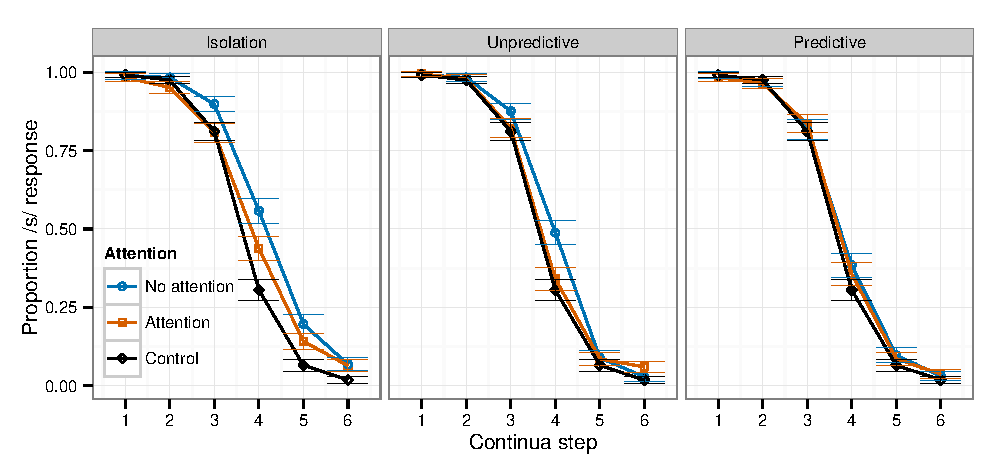
\includegraphics[width=\textwidth]{graphs/exp23_categresults}
\end{center}
\end{figure*}


As an additional comparison, the data from this experiment was combined with the subset of participants in Experiment 1 who were exposed to the same set of words (the word-medial condition).  
Exposure Type was recoded as a three-level factor, using treatment (dummy) contrast coding, with the Experiment 1 exposure (Isolation) as the reference level. 
An identically specified logistic mixed effects model was fit to this data set as to the initial data.  
In this model, there was a significant effect of Attention ($\beta = 0.74, SE = 0.32, z = 2.2, p = 0.02$), such that participants in Attention conditions were less likely to categorize the continua steps as /s/.  
Exposure Type had a marginal effect of Predictive compared to Isolation ($\beta = -0.43, SE = 0.23, z = -1.9, p = 0.05$), indicating that participants in the Predictive condition were less likely to categorize the continua as /s/ overall as compared to participants from Experiment 2. 
Step interacted with both Unpredictive as compared to Isolation ($\beta = -0.42, SE = 0.17, z = -2.4, p = 0.01$) and Predictive as compared to Isolation ($\beta = -0.32, SE = 0.14, z = -2.2, p = 0.02$).
These interactions indicate that the categorization functions for sentential stimuli had a steeper cross-over than the Isolation. 
As shown in Figure~\ref{fig:exp23categ}, the endpoints (Steps 5 and 6) for the sentential conditions are wholly overlapping with the control categorization for those steps.
While participants in the Unpredictive condition showed a shifted category boundary, the perceptual learning affected less of the continua than for participants in the Isolation condition.

An additional model was run with the reference level for Exposure Type as Predictive to check whether participants in the Predictive condition showed perceptual learning effects at all.
In the model with Predictive as reference, the intercept is no longer significant ($\beta = 0.44, SE = 0.28, z = 1.5, p = 0.12$), indicating perceptual learning was not robustly present in participants in the Predictive condition.  
The difference between the Predictive condition and the Isolation condition remains ($\beta = 0.77, SE = 0.32, z = 2.4, p = 0.01$), and, as above, the difference between Predictive and Unpredictive is not significant ($\beta = 0.42, SE = 0.31, z = 1.3, p = 0.17$).
These results indicate participants in the Predictive condition showed no perceptual learning effects, and participants in the Unpredictive condition were in between Predictive and Isolation, but not significantly different from either.  
Increasing the statistical power would be necessary to separate the conditions out further.


\section{Discussion}

The key finding of the current experiment is that modified categories embedded in words in meaningful sentences produce less perceptual learning than words in isolation.  
In fact, participants exposed to a modified category only in predictive words had a similar boundary as those in the control experiment who had no exposure to a modified /s/ category.
This pattern of results aligns the most with the extension to Kraljic and colleagues' argument that perceptual learning is a last resort.
If there is any way to attribute the acoustic atypicality to either linguistic or other sources of variation, no perceptual learning occurs \citep{Kraljic2008,Kraljic2008a}.
In the current experiment, semantic predictability may be a linguistic source of variation and shows similar effects as a more local source like consonant cluster coarticulation.

The prediction of a simple predictive coding model \citep{Clark2013} was not borne out.
Rather than increased expectations enhancing error signals, the conditions with increased expectations showed no perceptual learning at all.
How can we reconcile then the predictive coding model and the findings of the current experiment?
One way, certainly, is to incorporate the reliability argument of Kraljic and colleagues.
Bayesian approaches capture uncertainty quite well, so the unreliable tokens, such as those in the high predictability sentences, would have greater uncertainty associated with them.
Another possibility is that perceptual learning did occur, but it was not generalized to the test items.
Participants could have learned from their exposure how the speaker produces /s/ in high predictability contexts, but the context of words in isolation was too different from the exposure context.
Put another way, the participants could have learned how the speaker reduces his /s/ category, but not how the speaker normally produces it.

\begin{figure*}[!ht]
\centering
\caption{Schema of category relaxation in predictable sentences.  The solid vertical line represents the mean of the modified category similar to the one used for Experiment 1, and a dashed vertical line represents the mean of the Experiment 2 modified category.  A more atypical category, as was used in Experiment 2, has a higher probability of being categorized as /s/ in predictable sentences than in isolation.}
\label{fig:distPred}
\begin{center}
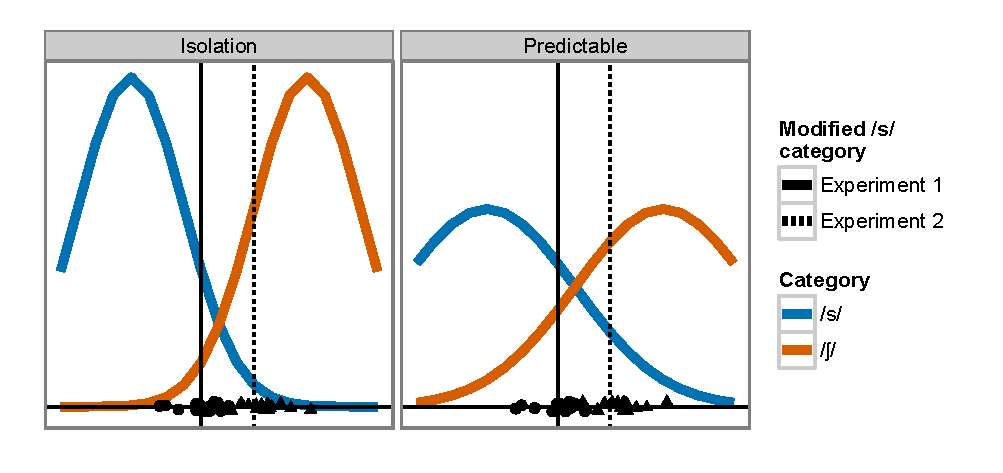
\includegraphics[width=\textwidth]{graphs/distPred}
\end{center}
\end{figure*}

However, if semantic predictability functions in a similar way as consonant cluster coarticulation, listeners would not show perceptual learning effects even if they were tested on a continuum in a high predictability sentence.
In \citet{Kraljic2008a}, listeners exposed to an ambiguous /s/ in the context of /st\textturnr/ and then tested on a continuum from /ast\textturnr i/ to /a\textesh t\textturnr i/ showed no perceptual learning effects.
Participants who were exposed to ambiguous /s/ intervocalically showed perceptual learning on both /asi/-/a\textesh i/ and /ast\textturnr i/-/a\textesh t\textturnr i/ continua.
There was no exposure-specificity effect, so participants do not even learn that the speaker produces a more /\textesh/-like /s/ in that context.
Any abstract encoding process accounts for and removes the variability associated with the context, leaving the unmodified perceptual category.
A similar pattern is likely to be seen with high predictability exposure.

One question raised by this finding is whether perceptual learning is possible at all in high predictability sentences.
If the range of acceptable variation for all categories is expanded (schematized in Figure~\ref{fig:distPred}), the modified category would have fallen closer to the expected mean in predictable sentences compared to isolation.
In terms of error propagation, the modified categories used here may not have generated enough errors to learn from.
Presenting listeners with a more atypical category should then cause more perceptual learning in this case.
In Figure~\ref{fig:distPred}, the atypical category from Experiment 2 would have a higher likelihood of being categorized as /s/ in predictable sentences than in isolation.
If increasing the atypicality in predictable sentences did in fact result in increased perceptual learning, it would suggest that perceptual learning is maximized in a particular range.
Tokens too close to the expected mean are too typical to learn from, and tokens too far from the expected mean are too unreliable.
However, if listeners simply ignore atypical sounds in highly predictable words, then increasing the atypicality of the category (i.e. using the ambiguity threshold from Experiment 2) would not increase perceptual learning.
If that were the case, listeners might not even be sensitive to replacing the /s/ with another sound category entirely (i.e. /f/) in a comprehension-oriented task \citep[but see][]{Samuel1981}.


\begin{figure*}[!ht]
\centering
\caption{Distribution of cross-over points for each participant across comparable exposure tokens in Experiments 1 and 3.}
\label{fig:exp13xoverdist}
\begin{center}
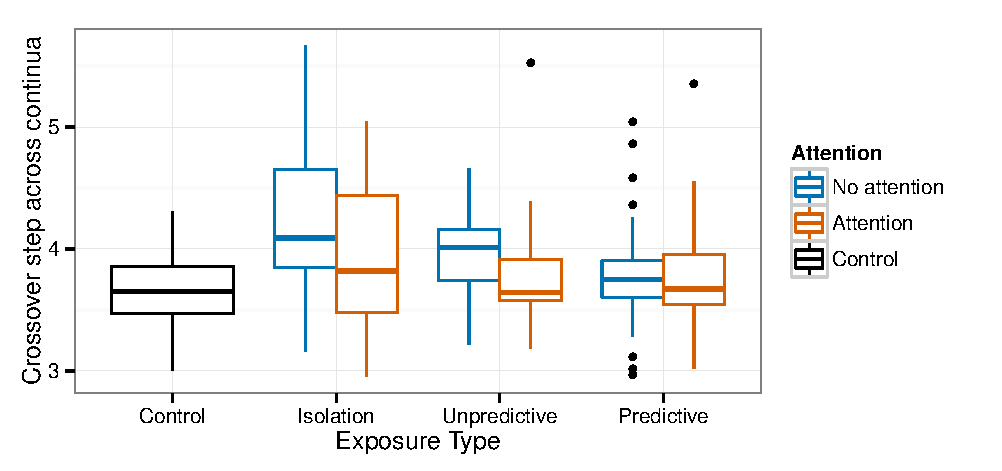
\includegraphics[width=\textwidth]{graphs/exp13_xoverdist}
\end{center}
\end{figure*}

As a final point in this discussion, the distribution of individuals' perceptual learning effects differs in shape as compared to Experiment 1. 
Figure~\ref{fig:exp13xoverdist} shows the distribution of cross-over points of each subject in Experiment 3 and participants in the condition of Experiment 1 that used the same exposure words.  
Cross-over points are where along the continua perception switches from primarily /s/ to primarily /\textesh/, and higher cross-over points are indicative of greater perceptual learning.
Participants exposed to the modified category in sentences show more consistency (larger bulges in the violin plots) than those exposed in isolated words.
In the Isolation conditions, participants follow a fairly wide, even distribution.
In contrast, participants in the sentence conditions a more tightly clustered either around the normalized cross over point or a step above, suggesting potentially discrete groups in the distribution.

One possible reason for these more discrete groups may relate to cognitive load.
Under lower cognitive load conditions, participants in perception-oriented tasks show greater perceptual sensitivity.
In this experiment, the task is comprehension-oriented, so lower cognitive load could have distributed cognitive resources either to the comprehension task or to aspects of the signal.
Participants with better attention-switching control might devote those resources to perception, while those with worse attention-switching control might not, revealing a relationship as was found in \citet{Scharenborg2013}.
Future research should quantify participants' attention-switching abilities and other individual differences that may play a role in explaining these findings.




%% The following is a directive for TeXShop to indicate the main file
%%!TEX root = diss.tex

\chapter{Conclusions}


\section{Effect of increased bias}

Bias for a word was manipulated in two ways, through position of the ambiguous sound in the word and through sentential manipulations.  Increased lexical bias resulted in 


\section{Specificity versus generalization}

In Experiment 1, greater perceptual learning was shown by participants exposed to ambiguous sounds later in the words, not to those at the beginnings of words

And yet, the testing continua consisted of stimuli with the sibilant at the beginnings of words, which are more similar to the S-Initial words than the S-Final words

Attention removed this effect of position, with the perceptual learning effect identical across participants in the exposure condition when they were told to pay attention to the sibilant

\section{Distance to canonical}

In Experiment 2, there was no effect of attention or lexical bias on perceptual learning, with a stable effect present for all listeners

There are two potential explanations for the lack of effects:

One, the increased distance to the canonical production increased the salience of the production and drew the listener's attention to the ambiguous productions, resulting in a similar pattern for listeners in Experiment 1 in the Attention condition

Two, the productions farther from canonical produce a weaker effect on the updating of a listener's categories

\begin{itemize}
\item Predicted by a Pierrehumbert model

\item This is supported somewhat by the weaker correlation between word endorsement rate and crossover point found in Experiment 2
	
\item Also supported by the findings of \citet{Sumner2011} where the most perceptual learning was found when the categories begin like the listener expects and gradually shift toward the speaker's actual boundaries over the course of exposure
\end{itemize}



%    3. Notes
%    4. Footnotes

%    5. Bibliography
\begin{singlespace}
\raggedright
\bibliographystyle{apalike}
\bibliography{biblio}
\end{singlespace}

\appendix
%    6. Appendices (including copies of all required UBC Research
%       Ethics Board's Certificates of Approval)
%\include{reb-coa}	% pdfpages is useful here
%\chapter{Supporting Materials}

This would be any supporting material not central to the dissertation.
For example:
\begin{itemize}
\item Authorizations from Research Ethics Boards for the various
    experiments conducted during the course of research.
\item Copies of questionnaires and survey instruments.
\end{itemize}


Ambiguous stimuli steps for experiments

Experiment 1

\begin{tabular}

Type & Word & Step chosen & Proportion /s/ response \\
Initial & ceiling & 7 & 0.40 \\
Initial & celery & 7 & 0.30 \\
Initial & cement & 7 & 0.26 \\
Initial & ceremony & 7 & 0.44 \\
Initial & saddle & 8 & 0.25 \\
Initial & safari & 6 & 0.45 \\
Initial & sailboat & 7 & 0.35 \\
Initial & satellite & 7 & 0.45 \\
Initial & sector & 6 & 0.39 \\
Initial & seminar & 7 & 0.33 \\
Initial & settlement & 7 & 0.42 \\
Initial & sidewalk & 7 & 0.30 \\
Initial & silver & 7 & 0.21 \\
Initial & socket & 7 & 0.30 \\
Initial & sofa & 7 & 0.26 \\
Initial & submarine & 7 & 0.45 \\
Initial & sunroof & 6 & 0.39 \\
Initial & surfboard & 7 & 0.59 \\
Initial & syrup & 6 & 0.37 \\
Final & carousel & 7 & 0.45 \\
Final & castle & 7 & 0.50 \\
Final & concert & 7 & 0.53 \\
Final & croissant & 7 & 0.42 \\
Final & currency & 7 & 0.58 \\
Final & cursor & 8 & 0.53 \\
Final & curtsy & 8 & 0.40 \\
Final & dancer & 7 & 0.45 \\
Final & dinosaur & 7 & 0.50 \\
Final & faucet & 7 & 0.45 \\
Final & fossil & 8 & 0.30 \\
Final & galaxy & 9 & 0.47 \\
Final & medicine & 8 & 0.55 \\
Final & missile & 10 & 0.30 \\
Final & monsoon & 8 & 0.42 \\
Final & pencil & 7 & 0.45 \\
Final & pharmacy & 8 & 0.42 \\
Final & tassel & 8 & 0.35 \\
Final & taxi & 8 & 0.50 \\
Final & whistle & 7 & 0.58 \\
 &  & 7.26 & 0.41 \\

\end{tabular}

Experiment 2

\begin{tabular}

Type & Word & Step chosen & Proportion /s/ response \\
Initial & ceiling & 8 & 0.20 \\
Initial & celery & 7 & 0.30 \\
Initial & cement & 7 & 0.26 \\
Initial & ceremony & 8 & 0.39 \\
Initial & saddle & 8 & 0.25 \\
Initial & safari & 7 & 0.21 \\
Initial & sailboat & 7 & 0.35 \\
Initial & satellite & 8 & 0.30 \\
Initial & sector & 6 & 0.39 \\
Initial & seminar & 7 & 0.33 \\
Initial & settlement & 8 & 0.35 \\
Initial & sidewalk & 7 & 0.30 \\
Initial & silver & 7 & 0.21 \\
Initial & socket & 7 & 0.30 \\
Initial & sofa & 7 & 0.26 \\
Initial & submarine & 9 & 0.32 \\
Initial & sunroof & 6 & 0.39 \\
Initial & surfboard & 8 & 0.25 \\
Initial & syrup & 6 & 0.37 \\
Final & carousel & 8 & 0.25 \\
Final & castle & 9 & 0.25 \\
Final & concert & 10 & 0.30 \\
Final & croissant & 8 & 0.20 \\
Final & currency & 9 & 0.30 \\
Final & cursor & 11 & 0.30 \\
Final & curtsy & 9 & 0.26 \\
Final & dancer & 8 & 0.26 \\
Final & dinosaur & 9 & 0.39 \\
Final & faucet & 8 & 0.25 \\
Final & fossil & 8 & 0.30 \\
Final & galaxy & 10 & 0.26 \\
Final & medicine & 9 & 0.30 \\
Final & missile & 10 & 0.30 \\
Final & monsoon & 9 & 0.15 \\
Final & pencil & 8 & 0.37 \\
Final & pharmacy & 9 & 0.39 \\
Final & tassel & 8 & 0.35 \\
Final & taxi & 10 & 0.35 \\
Final & whistle & 9 & 0.35 \\
 &  & 8.1282051282 & 0.2978782426 \\

\end{tabular}

\backmatter
%    7. Index
% See the makeindex package: the following page provides a quick overview
% <http://www.image.ufl.edu/help/latex/latex_indexes.shtml>


\end{document}
